% !TeX encoding = UTF-8
% !TeX program = xelatex
% !TeX spellcheck = en_US

\documentclass[degree=master,language=chinese,font=external,cjk-font=external]{sustechthesis}
  %%%%%%%%%%%%%%%%%%%%%%%%%%%%%%%%%%%%%%%
  %   研究生报告模板:开题报告,年度考核报告
  %%%%%%%%%%%%%%%%%%%%%%%%%%%%%%%%%%%%%%%

  % 学位 degree:
  %   master (默认) | doctor
  % 语言 language:
  %   chinese (默认)| english
  % 英文字体 font
  %   auto (默认,自动选择系统自带字体)| external (包内字体)| times | termes | 等
  %   Windows 和 macOS 系统上,无需设定。系统自带对应字体,可以删除该参数。
  %   Unix 系统推荐使用包内字体,而非TeX自带的克隆版字体,以达到和其他系统一致的字体效果。
  %   Windows 系统上可以删除该参数,使用系统内置字体。
  % 中文字体 cjk-font
  %   auto (默认,自动选择系统自带字体)| external (包内字体)| windows | mac | 等
  %   在 **非Windows** 的系统上推荐使用包内字体,而非系统字体。
  %   以达到和 Windows 系统一致的字体效果。
  %   Windows 系统自带对应字体,可以删除该参数。

  
% 论文基本配置,加载宏包等全局配置
% 在此文件中可以选择
% 1. 【重要】文档类型(开题报告,年度考核报告),默认不开启该选项。
% 2. 生成的PDF为无空白页的用于电子版提交的版本 或 插入空白页的以便双面打印的版本
% 3. 学位学科门类(理学、工学、医学)
% 4. 培养单位
% 5. 作者姓名、指导教师等
% !TeX root = ./sustechthesis-example.tex

% 论文基本信息配置

\thusetup{
  %******************************
  % 注意:
  %   1. 配置里面不要出现**空行**
  %   2. 不需要的配置信息可以删除
  %   3. 建议先阅读文档中所有关于选项的说明
  %******************************
  %
  % 输出格式
  %   选择打印版(print)或用于提交的电子版(electronic),前者会插入空白页以便直接双面打印
  %
  output = electronic,
  %
  % 文档类型
  %   选择开题报告(proposal)、年度考核报告(progress)或学位论文(thesis)【默认值】。
  %
  type = proposal,
  %
  % 标题
  %   可使用“\\”命令手动控制换行
  %   如果需要使用副标题,取消 subtitle 和 subtitle* 的注释即可。
  %   特别字符允许小写,例如行内公式,其他所有字词全部大写。
  %
  title  = {足式机器人强化学习控制调研},
  % title* = {机械狗经典控制、RL控制},
  subtitle = {机械狗经典控制、RL控制},
  % subtitle* = {optional subtitle optional subtitle optional subtitle optional subtitle optional subtitle optional subtitle},
  %
  % 学位
  %
  degree-domain = {工学}, % 【中文】学科门类:可选理学、工学、医学
  degree-domain* = {Engineering}, % 【英文】学位等级:可选Science, Engineering, Medicine
  gongshuo = false, % 是否为专业型学位。专业型学位则填 true ,学术型或其他为 false 。
  %
  % 培养单位
  %   填写所属院系的全名
  %   超长英文系名可以手动换行
  department = {计算机科学与工程系},
  department* = {School of System Design and \\Intelligent Manufacturing},
  %
  % 学科
  %   1. 学术型学位
  %      获得一级学科授权的学科填写一级学科名称,其他填写二级学科名称
  %   2. 工程硕士
  %      工程领域名称
  %
  discipline  = {计算机科学与技术},
  discipline* = {Computer Science and Technology},
  %
  % 姓名
  %   英文用全拼,姓在前,名在后,姓和名的首字母大写,其余小写
  %
  author-id  = {11900000},
  author  = {彭道杰},
  author* = {PENG Daojie},
  %
  % 指导教师
  %   一般情况下,只写一名指导教师。
  %   填写导师姓名,后衬导师职称“教授”,“副教授”,“研究员”等
  %
  supervisor  = {爱丽丝鲍勃助理教授},
  supervisor* = {Assistant Prof. Alice Bob},
  % 副指导教师
  %   一般无需启用该项,留空或者注释掉即可。
  %   如需启用限填写一名,且需要向学位办确认和备案,职称要求同指导教师。
  % associate-supervisor  = {大卫查理助理教授},
  % associate-supervisor* = {Assistant Prof. David Charlie},
  %
  % 日期
  %   使用 ISO 格式;默认为当前时间
  %   date 为第一页全中文大写日期,defense-date 为第二、三页的答辩日期。
  %   需要按 {年-月-日} 格式填写,如不显示“日”,可以随意填一个日期,但是不能为空。
  %
  date = {2020-12-20},
  defense-date = {2020-12-20},
  %
  % 密级
  %   公开, 秘密, 机密, 绝密
  %
  statesecrets={公开},
  %
  % 国内图书分类号:查询网址:https://ztflh.xhma.com/
  %   国内图书分类号可先参考知网上类似学位论文的分类号,再进行确认。
  % 国际图书分类号,查询网址:https://udcsummary.info/php/index.php?lang=chi
  %
  natclassifiedindex={XXxxx.x},
  intclassifiedindex={xx-x},
}


\thusetup{
  %
  % 数学字体
  % math-style = GB,  % GB (中文默认) | TeX (英文默认)
  math-font  = cambria,  % cambria (默认,同 Word 默认数学字体一致) | times (Times New Roman 的TeX克隆版)| xits | stix
}

% 载入所需的宏包

% 可以使用 nomencl 生成符号和缩略语说明
% \usepackage{nomencl}
% \makenomenclature

% 表格加脚注
\usepackage{threeparttable}

% 表格中支持跨行
\usepackage{multirow}

% 量和单位
\usepackage{siunitx}

% 定理类环境宏包
\usepackage{amsthm}
% 也可以使用 ntheorem
% \usepackage[amsmath,thmmarks,hyperref]{ntheorem}

%%%%%% 顺序编码制的文献引用形式
%%%%%% 参考文献编译方式二选一,不要同时开启。
%%%% 选择一:使用 BibTeX + natbib 宏包
\usepackage[sort&compress]{gbt7714}
\citestyle{super} % 全局上标数字模式
% \citestyle{numbers} % 全局行内数字模式,在写作指南2022年8月23日版本已废弃, 并决定中英文都采用上标数字格式
\bibliographystyle{sustechthesis-numeric}

%%%% 选择二:使用 BibLaTeX 宏包(兼容性不佳,不太推荐)
% \usepackage[backend=biber,style=gb7714-2015,gbalign=left]{biblatex}
% \addbibresource{ref/refs.bib} % 声明 BibLaTeX 的数据库

% 定义所有的图片文件在 figures 子目录下
\graphicspath{{figures/}}

% 数学命令
\newcommand\dif{\mathop{}\!\mathrm{d}}  % 微分符号

% hyperref 宏包在最后调用
\usepackage{hyperref}
\usepackage{ragged2e}

% 固定宽度的表格。放在 hyperref 之前的话,tabularx 里的 footnote 显示不出来。
\usepackage{tabularx}

% 跨页表格,必须在 hyperref 之后使用否则会报错。
\usepackage{longtable}

% % 源代码 minted 高亮,二选一即可。【不再推荐,会有兼容性问题:导致图表间距异常】
% %% 使用 minted 包有内置高亮颜色,需要 Python 环境编译,并安装 Pygement 包。
% \usepackage{minted}

% 源代码 listings 高亮,二选一即可。
\usepackage{listings}
%% 使用 listings 包需要自行定义高亮颜色,此处给出 Java 的例子。
\definecolor{javared}{rgb}{0.6,0,0} % for strings
\definecolor{javagreen}{rgb}{0.25,0.5,0.35} % comments
\definecolor{javapurple}{rgb}{0.5,0,0.35} % keywords
\definecolor{javadocblue}{rgb}{0.25,0.35,0.75} % javadoc

\lstset{language=Java,
  keywordstyle=\color{javapurple}\bfseries,
  stringstyle=\color{javared},
  commentstyle=\color{javagreen},
  morecomment=[s][\color{javadocblue}]{/**}{*/},
  numbers=left,
  numberstyle=\tiny\color{black},
  stepnumber=1,
  numbersep=10pt,
  tabsize=4,
  showspaces=false,
  showstringspaces=false
}

% 伪代码环境
\usepackage[ruled,linesnumbered]{algorithm2e}
% 定义伪代码的continue
\SetKw{Continue}{continue}
\SetKw{Break}{break}
% 定义算法注释
\SetKwComment{Comment}{/* }{ */}
\SetKwComment{SingleComment}{// }{}
\SetKwComment{TriComment}{$\triangleright$\ }{}

% tabular 扩展命令
\newcolumntype{R}[1]{>{\raggedleft\arraybackslash}p{#1}} % 定义R为表格左右居左,用于自定义表格列宽度
\newcolumntype{L}[1]{>{\raggedright\arraybackslash}p{#1}} % 定义L为表格左右居右,用于自定义表格列宽度
\newcolumntype{C}[1]{>{\centering\arraybackslash}p{#1}} % 定义C为表格左右居中,用于自定义表格列宽度

% tabularx 扩展命令,会对单元格内容进行单元格内自动换行
% X 默认就是两端对齐
% Y 左对齐
\newcolumntype{Y}{>{\raggedright\arraybackslash}X}
% Z 右对齐
\newcolumntype{Z}{>{\raggedleft\arraybackslash}X}
% A 居中对齐
\newcolumntype{A}{>{\centering\arraybackslash}X}

% 表格旋转
\usepackage{rotating}


\newcommand\undefcolumntype[1]{\expandafter\let\csname NC@find@#1\endcsname\relax}
\newcommand\forcenewcolumntype[1]{\undefcolumntype{#1}\newcolumntype{#1}}


\begin{document}

% 封面
\maketitle

\frontmatter
% !TeX root = ../sustechthesis-example.tex

% 中英文摘要和关键字

\begin{abstract}
  足式机器人相对于常见的轮式和履带式机器人有着更加灵活,环境适应能力强的优势。与启发它们的人类或者动物一样,这类机器人拥有着更强的越野能力,能够适应复杂的地形环境,到达普通轮式或履带式机器人无法到达的地方。然而,这类机器人往往具有更多的自由度,这使得对它们的控制变得具有挑战性。如何让这类足式机器人像它们的动物模仿对象一样能够灵活、优雅地运动成为一个重要的研究课题。在这其中,模仿四足动物的四足机器人(机械狗)是一类被广泛研究的对象。

  机械狗



  % 关键词用“英文逗号”分隔,输出时会自动处理为正确的分隔符
  \thusetup{
    keywords = {机器人控制, 轨迹优化, 深度学习, 强化学习控制, Isaac仿真},
  }
\end{abstract}

% \begin{abstract*}
%   An abstract of a dissertation is a summary and extraction of research work and contributions.
%   Included in an abstract should be description of research topic and research objective, brief introduction to methodology and research process, and summarization of conclusion and contributions of the research.
%   An abstract should be characterized by independence and clarity and carry identical information with the dissertation.
%   It should be such that the general idea and major contributions of the dissertation are conveyed without reading the dissertation.

%   An abstract should be concise and to the point.
%   It is a misunderstanding to make an abstract an outline of the dissertation and words “the first chapter”, “the second chapter” and the like should be avoided in the abstract.

%   For thesis written in \textbf{Chinese} as the main text, the abstract of doctoral thesis is about 800 to 1000 words; and the abstract of the master's thesis is generally about 500 words; the length is limited to one page.
%   For thesis written in \textbf{English} as the main text, the word count of Chinese abstracts is required to be 800 to 1000 words (regardless doctoral thesis or master's thesis).

%   The abstract of the doctoral thesis is about 800 to 1000 words; the abstract of the master's thesis is generally about 500 words; the length is limited to one page.

%   Keywords are terms used in a dissertation for indexing, reflecting core information of the dissertation.
%   An abstract may contain a maximum of 5 keywords, with semi-colons used in between to separate one another.

%   % Use comma as seperator when inputting
%   \thusetup{
%     keywords* = {keyword 1, keyword 2, keyword 3, keyword 4, looooooooooooooooooooong keyword 5},
%   }
% \end{abstract*}

% 目录
\tableofcontents

% 插图和附表清单
% \listoffiguresandtables  % 插图和附表清单
% \listoffigures           % 插图清单
% \listoftables            % 附表清单

% 符号对照表(非强制性要求,如果论文中所用符号不多,可以略去)
% % !TeX root = ../sustechthesis-example.tex

% denotation 环境带一个可选参数,用来指定符号列的宽度(默认为 2.5cm),下面改3cm为例。
% 如果论文中使用了大量的物理量符号、标志、缩略词、专门计量单位、自定义名词和术语等, 应编写“符号和缩略语说明”。
% 论文中主要符号应全部采用法定单位, 严格执行《量和单位》(GB3100~3102-93)的有关规定、单位名称的书写,可以采用国际通用符号,也可以用中文名称,但全文应统一,不得两种混用。
% 缩略语应列出中英文全称。符号和缩略语说明排序方法先按拉丁字母大写、小写排序, 再按希腊字母大写、小写排序, 如下表所示:
% ABCDEFGHIJKLMNOPQRSRUVWXYZ
% abcdefghijklmnopqrstuvwxyz
% Alpha
% Beta
% Gamma
% Delta
% Epsilon
% Zeta
% Eta
% Theta
% Iota
% Kappa
% Lambda
% Mu
% Nu
% Xi
% Omicron
% Pi
% Rho
% Sigma
% Tau
% Upsilon
% Phi
% Chi
% Psi
% Omega
% alpha
% beta
% gamma
% delta
% epsilon
% zeta
% eta
% theta
% iota
% kappa
% lambda
% mu
% nu
% xi
% omicron
% pi
% rho
% sigma
% tau
% upsilon
% phi
% chi
% psi
% omega

% 希腊字母详见 https://xilazimu.net/


\begin{denotation}[3cm]
  \item[As-PPT]聚苯基不对称三嗪
  \item[DFT]密度泛函理论 (Density Functional Theory)
  \item[DMAsPPT]聚苯基不对称三嗪双模型化合物(水解实验模型化合物)
  \item[$E_a$]化学反应的活化能 (Activation Energy)
  \item[HMAsPPT]聚苯基不对称三嗪模型化合物的质子化产物
  \item[HMPBI]聚苯并咪唑模型化合物的质子化产物
  \item[HMPI]聚酰亚胺模型化合物的质子化产物
  \item[HMPPQ]聚苯基喹噁啉模型化合物的质子化产物
  \item[HMPY]聚吡咙模型化合物的质子化产物
  \item[HMSPPT]聚苯基对称三嗪模型化合物的质子化产物
  \item[HPCE]高效毛细管电泳色谱 (High Performance Capillary lectrophoresis)
  \item[HPLC]高效液相色谱 (High Performance Liquid Chromatography)
  \item[IRC]内禀反应坐标 (Intrinsic Reaction Coordinates)
  \item[LC-MS]液相色谱-质谱联用 (Liquid chromatography-Mass Spectrum)
  \item[MAsPPT]聚苯基不对称三嗪单模型化合物,3,5,6-三苯基-1,2,4-三嗪
  \item[MPBI]聚苯并咪唑模型化合物,N-苯基苯并咪唑
  \item[MPI]聚酰亚胺模型化合物,N-苯基邻苯酰亚胺
  \item[MPPQ]聚苯基喹噁啉模型化合物,3,4-二苯基苯并二嗪
  \item[MPY]聚吡咙模型化合物
  \item[MSPPT]聚苯基对称三嗪模型化合物,2,4,6-三苯基-1,3,5-三嗪
  \item[ONIOM]分层算法 (Our own N-layered Integrated molecular Orbital and molecular Mechanics)
  \item[PBI]聚苯并咪唑
  \item[PDT]热分解温度
  \item[PES]势能面 (Potential Energy Surface)
  \item[PI]聚酰亚胺
  \item[PMDA-BDA]均苯四酸二酐与联苯四胺合成的聚吡咙薄膜
  \item[PPQ]聚苯基喹噁啉
  \item[PY]聚吡咙
  \item[S-PPT]聚苯基对称三嗪
  \item[SCF]自洽场 (Self-Consistent Field)
  \item[SCRF]自洽反应场 (Self-Consistent Reaction Field)
  \item[TIC]总离子浓度 (Total Ion Content)
  \item[TS]过渡态 (Transition State)
  \item[TST]过渡态理论 (Transition State Theory)
  \item[ZPE]零点振动能 (Zero Vibration Energy)
  \item[\textit[ab initio]]基于第一原理的量子化学计算方法,常称从头算法
  \item[$\Delta G^\neq$]活化自由能(Activation Free Energy)
  \item[$\kappa$]传输系数 (Transmission Coefficient)
  \item[$\nu_i$]虚频 (Imaginary Frequency)
\end{denotation}



% 也可以使用 nomencl 宏包,需要在导言区
% \usepackage{nomencl}
% \makenomenclature

% 在这里输出符号说明
% \printnomenclature[3cm]

% 在正文中的任意为都可以标题
% \nomenclature{As-PPT}{聚苯基不对称三嗪}
% \nomenclature{DFT}{密度泛函理论 (Density Functional Theory)}
% \nomenclature{DMAsPPT}{聚苯基不对称三嗪双模型化合物(水解实验模型化合物)}
% \nomenclature{$E_a$}{化学反应的活化能 (Activation Energy)}
% \nomenclature{HMAsPPT}{聚苯基不对称三嗪模型化合物的质子化产物}
% \nomenclature{HMPBI}{聚苯并咪唑模型化合物的质子化产物}
% \nomenclature{HMPI}{聚酰亚胺模型化合物的质子化产物}
% \nomenclature{HMPPQ}{聚苯基喹噁啉模型化合物的质子化产物}
% \nomenclature{HMPY}{聚吡咙模型化合物的质子化产物}
% \nomenclature{HMSPPT}{聚苯基对称三嗪模型化合物的质子化产物}
% \nomenclature{HPCE}{高效毛细管电泳色谱 (High Performance Capillary lectrophoresis)}
% \nomenclature{HPLC}{高效液相色谱 (High Performance Liquid Chromatography)}
% \nomenclature{IRC}{内禀反应坐标 (Intrinsic Reaction Coordinates)}
% \nomenclature{LC-MS}{液相色谱-质谱联用 (Liquid chromatography-Mass Spectrum)}
% \nomenclature{MAsPPT}{聚苯基不对称三嗪单模型化合物,3,5,6-三苯基-1,2,4-三嗪}
% \nomenclature{MPBI}{聚苯并咪唑模型化合物,N-苯基苯并咪唑}
% \nomenclature{MPI}{聚酰亚胺模型化合物,N-苯基邻苯酰亚胺}
% \nomenclature{MPPQ}{聚苯基喹噁啉模型化合物,3,4-二苯基苯并二嗪}
% \nomenclature{MPY}{聚吡咙模型化合物}
% \nomenclature{MSPPT}{聚苯基对称三嗪模型化合物,2,4,6-三苯基-1,3,5-三嗪}
% \nomenclature{ONIOM}{分层算法 (Our own N-layered Integrated molecular Orbital and molecular Mechanics)}
% \nomenclature{PBI}{聚苯并咪唑}
% \nomenclature{PDT}{热分解温度}
% \nomenclature{PES}{势能面 (Potential Energy Surface)}
% \nomenclature{PI}{聚酰亚胺}
% \nomenclature{PMDA-BDA}{均苯四酸二酐与联苯四胺合成的聚吡咙薄膜}
% \nomenclature{PPQ}{聚苯基喹噁啉}
% \nomenclature{PY}{聚吡咙}
% \nomenclature{S-PPT}{聚苯基对称三嗪}
% \nomenclature{SCF}{自洽场 (Self-Consistent Field)}
% \nomenclature{SCRF}{自洽反应场 (Self-Consistent Reaction Field)}
% \nomenclature{TIC}{总离子浓度 (Total Ion Content)}
% \nomenclature{TS}{过渡态 (Transition State)}
% \nomenclature{TST}{过渡态理论 (Transition State Theory)}
% \nomenclature{ZPE}{零点振动能 (Zero Vibration Energy)}
% \nomenclature{\textit{ab initio}}{基于第一原理的量子化学计算方法,常称从头算法}
% \nomenclature{$\Delta G^\neq$}{活化自由能(Activation Free Energy)}
% \nomenclature{$\kappa$}{传输系数 (Transmission Coefficient)}
% \nomenclature{$\nu_i$}{虚频 (Imaginary Frequency)}



% 正文部分
\mainmatter
% !TeX root = ../sustechthesis-example.tex

\chapter[基于质心动力学(Centroidal Dynamics)模型的TO控制]{基于质心动力学(Centroidal Dynamics)模型的TO控制}

足式机器人的运动规划是比较困难的,不仅因为它的自由度较多,更因为它的机体运动不能被直接得出,而是要通过四肢状态及四肢与环境的接触产生。

经典控制的基础是对机器人的运动学和动力学建模。经典控制主要方式有\emph{轨迹优化(Trajectory Optimization, TO)}和\emph{模型预测控制(Model Predictive Control, MPC)}两类。常用的\emph{轨迹优化}机械狗动力模型有两种\cite[p2]{Winkler_Bellicoso_Hutter_Buchli_2018}:\emph{1. 基于质心动力学的模型;2. 基于直接刚体动力学的模型}。基于这些模型的优化控制都被描述为\emph{非线性优化问题},这些问题的求解算力开销较大往往不能够在线完成,需要上位机的辅助。


% \section[基于质心动力学模型(Centroidal Dynamics)的TO控制]{基于质心动力学模型(Central Dynamics)的TO控制\cite[p2-5]{Bellicoso_Jenelten_Fankhauser_Gehring_Hwangbo_Hutter_2017}}
% \textcolor{red}{\small
% 基于参考文献阐述基于ZMP方法,质心动力学模型的控制方法...
% }



\section[机械狗的运动模型(Motion Model)]{\label{section:motion_model}机械狗的运动模型(Motion Model)\cite[p2]{Bellicoso_Jenelten_Fankhauser_Gehring_Hwangbo_Hutter_2017, Bellicoso_Jenelten_Gehring_Hutter_2018}}

机器人与环境接触的机械系统的运动模型描述方程可以描述如下:

\begin{align}
    {\mathbfit M}({\mathbfit q})\dot{\mathbfit u} + {\mathbfit h}({\mathbfit q}, {\mathbfit u}) =  {\mathbfit S}^T{\mathbfit \tau} + {\mathbfit J}_S^T {\mathbfit \lambda}
\end{align}
这其中${\mathbfit q}$是一个描述机器人主体及各个节点的广义位置矢量:
\begin{align}
    {\mathbfit q}= \begin{bmatrix}_I {\mathbfit r}_{IB} \\ {\mathbfit q}_{IB} \\ {\mathbfit q}_j\end{bmatrix} \in SE(3)\times {\mathbb R}^{n_j}
\end{align}

它里面$_I {\mathbfit r}_{IB} \in {\mathbb R}^{3}$是机器人主体相对于惯性系的三维位置矢量;${\mathbfit q}_{IB} \in SO(3)$是机器人主体相对于惯性系的转动描述,用哈密顿单位四元数表示的;${\mathbfit q}_j \in {\mathbb R}^{n_j}$是一个储存机器人所有节点角度的$n_j$维矢量。


这其中${\mathbfit u}$是一个描述机器人主体及各个节点的广义速度矢量:
\begin{align}
    {\mathbfit u}= \begin{bmatrix}_I{\mathbfit v}_B \\ _B{\mathbfit \omega}_{IB} \\ \dot {\mathbfit q}_j \end{bmatrix} \in {\mathbb R}^{n_u} 
\end{align}

它里面的$_I{\mathbfit v}_B$描述了机器人主体相对于惯性系的速度;$_B{\mathbfit \omega}_{IB}$描述了机器人主体相对于自身的角速度;$\dot {\mathbfit q}_j$描述了机器人的各个关节转动的速度。
这其中${\mathbfit M}$是一个关于机器人整体的质量矩阵,它是一个$n_u \times n_u$的矩阵: 
\begin{align}
    {\mathbfit M} \in {\mathbb R}^{n_u \times n_u}
\end{align}

这个质量矩阵的具体数值跟机器人的机械系统的状态(各个节点的位置${\mathbfit q}$)相关,可以通过通用的方式计算出它的表达式。实际计算的时候只需要带入${\mathbfit q}$的值,就可以计算出${\mathbfit M}$矩阵的各个元素具体数值。
这其中${\mathbfit h}$是一个跟机器人的机械位置和速度都有关的量,包含了机械系统产生的克里奥利力、离心力和重力的作用,它是一个$n_u$维的矢量:
\begin{align}
    {\mathbfit h} \in {\mathbb R}^{n_u}
\end{align}

这其中${\mathbfit S}$是一个选择矩阵,可以用来选择整个公式中哪些自由度被激活,它是一个$n_{\tau} \times n_u$的矩阵:
\begin{align}
    {\mathbfit S} = \begin{bmatrix}{\mathbfit 0}_{n_{\tau} \times (n_u - n_{\tau})} & {\mathbb I}_{n_{\tau} \times n_{\tau}}\end{bmatrix} \in {\mathbb R}^{n_{\tau} \times n_u} 
\end{align}

它其中包含的参数$n_{\tau}$表示被激活的自由度数量,如果机器人的所有自由度都被激活,则$n_{\tau} = n_j$。
这其中${\mathbfit \tau}$是机器人各个关节的电机提供的扭矩,它是一个$n_j$维的向量:
\begin{align}
    {\mathbfit \tau} \in {\mathbb R}^{n_j} 
\end{align}

它的节点成员是否产生作用受到${\mathbfit S}^T$矩阵的选择。
这其中${\mathbfit J}_S$是一些列雅可比矩阵的集合:
\begin{align}
    J_S=\begin{bmatrix}J^T_{C_1} & ... & J^T_{C_{n_c}}\end{bmatrix}^T  \in {\mathbb R}^{3n_c\times n_u}
\end{align}

它是接触点的支撑力${\mathbfit \lambda}$向节点力转换的矩雅可比矩阵,包含了$n_c$个雅可比矩阵,$n_c$为接触地面的肢体个数。

如果足接触建模为点接触的话,在稳定接触的情况下,每个接触点会产生三个相应的约束条件:
\begin{align}
    \label{eq:contact_constrains}
    \begin{cases}
        _I\mathbfit{r}_{IC}(t)=const\\
        _I \mathbfit{\dot r}_{IC}=\mathbfit{J}_C\mathbfit{u}=0\\
        _I\mathbfit{\ddot r}_{IC}=\mathbfit{J}_C \mathbfit{\dot u}+\mathbfit{\dot J}_C\mathbfit{u}=0
    \end{cases}
\end{align}

其含义就是在惯性系下看接触点的位置是固定的为定值,并且其速度和加速,也即其一阶导数和二阶导数为零。











\section[分层次优化(Hierarchical Optimization)计算]{\label{section:hierarchical_opt}分层次优化(Hierarchical Optimization)计算\cite[p2]{Bellicoso_Jenelten_Fankhauser_Gehring_Hwangbo_Hutter_2017}}

整个优化计算过程的最终目的是得到一个扭矩参考目标${\mathbfit \xi}_d$用来作为输入控制电机,${\mathbfit \xi}_d$包含两部分信息:关节点的运动加速度$\mathbfit{\dot u}_d^T$和接触力$\mathbfit{\lambda}_d^T$。控制方法采用接触力控制,优化化计算的策略是采取分层次优化的方式。在这一部分我们将从\ref{section:motion_model}节中描述的运动模型出发,拆接触其中的内容进行分层次优化。我们将介绍运动方程、接触部分的运动约束、接触力和扭矩限制、运动跟随、接触力最小化、根据优化结果计算电机扭矩等内容。

\subsection[基体运动方程]{基体运动方程}
通过利用选择矩阵$\mathbfit{S}^T$诱导的分解,我们可以将运动和接触力限制在浮动基系统动力学描述的流形上,有如下式:
\begin{align}
    \begin{bmatrix}{\mathbfit M}_{fb} & - {\mathbfit J}_{s_{fb}}^T \end{bmatrix} {\mathbfit \xi}_d = - {\mathbfit h}_{fb}
\end{align}

这里$XXX_{fb}$:下标的意思是浮动的主体-'floating base',各个参数的具体含义解释如下:

\begin{enumerate}
    \item ${\mathbfit \xi}_d$是一个一个$n_u+n_c$行$1$列的向量: ${\mathbfit \xi}_d = \begin{bmatrix} {\mathbfit u}_d^T & {\mathbfit \lambda}_d^T \end{bmatrix} \in {\mathbb R}^{n_u+n_c}$,其中:
    \begin{enumerate}
        \item ${\mathbfit u}_d^T$是目标关节点的加速度;
        \item ${\mathbfit \lambda}_d^T$是目标接触力;
    \end{enumerate}
    \item ${\mathbfit M}_{fb}$是复合型惯性矩阵的前六行;
    \item ${\mathbfit J}_{s_{fb}}^T$是雅克比阵的前六行,它将接触力转换到节点的扭矩;
    \item ${\mathbfit h}_{fb}$是非线性项的前六行,包括克里奥利力、离心力和重力项;
\end{enumerate}

\subsection[地面接触部分运动约束]{地面接触部分运动约束}

控制器找到的解决方案不应违反\eqref{eq:contact_constrains}中定义的接触约束。因此,我们通过设置在接触点施加空加速度:
\begin{align}
    \begin{bmatrix} {\mathbfit J}_s & {\mathbfit 0}_{3n_c \times 3n_c}\end{bmatrix} {\mathbfit \xi}_d = - \dot {\mathbfit J}_s {\mathbfit u} 
\end{align}

它将${\mathbfit \xi}_d$带进去计算后就得到了:${\mathbfit J}_s  {\mathbfit \xi}_d  = - \dot {\mathbfit J}_s {\mathbfit u}$其实就是公式\eqref{eq:contact_constrains}的第二个式子${\mathbfit J}_s  {\mathbfit \xi}_d  + \dot {\mathbfit J}_s {\mathbfit u} = 0$。

\subsection[接触力限制]{接触力限制}

\begin{align}
    \begin{cases}
        \label{eq:friction_constrains}
        (_I{\mathbfit h} - {_I{\mathbfit n}}_{\mu})^T {_I{\mathbfit \lambda}}_k\leq & 0 \\
        - (_I{\mathbfit h} + {_I{\mathbfit n}}_{\mu})^T {_I{\mathbfit \lambda}}_k\leq & 0 \\
        (_I{\mathbfit l} - {_I{\mathbfit n}}_{\mu})^T {_I{\mathbfit \lambda}}_k\leq & 0 \\
        - (_I{\mathbfit l} + {_I{\mathbfit n}}_{\mu})^T {_I{\mathbfit \lambda}}_k\leq & 0
    \end{cases}
\end{align}

$_In$是接触面的法向量;$\mu$是摩擦系数;有了这两个再乘上受力$_I\lambda$,就可以得出最大静摩擦力$_I{\mathbfit n}_{\mu}^T \lambda$。实际在接触点平行于地面方向的两个分力$_I{\mathbfit h}$,$_I{\mathbfit l}$在正反方向上都不应该比这个值大,否则就会发生滑动。这就是公式\eqref{eq:friction_constrains}约束的由来。

\subsection[扭矩限制]{扭矩限制}
对于扭矩有如下约束:
\begin{align}
    \label{eq:torque_constrains}
    {\mathbfit \tau}_{min}-{\mathbfit h}_j 
    \leq \begin{bmatrix} {\mathbfit M}_j & -{\mathbfit J}^T_{s_j} \end{bmatrix} 
    \leq {\mathbfit \tau}_{max}-{\mathbfit h}_j 
\end{align}

这里的${\mathbfit h}_j$就是科里奥利力那一堆东西。
而$\begin{bmatrix} {\mathbfit M}_j & -{\mathbfit J}^T_{s_j} \end{bmatrix}$就是加速度力${\mathbfit M}_j  \dot{\mathbfit u}_d^T$和传递力$-{\mathbfit J}^T_{s_j} {\mathbfit \lambda}_d^T$两项的和。它们计算的结果就是电机提供的扭矩力${\mathbfit \tau}$克服完${\mathbfit h}({\mathbfit q}, {\mathbfit u})$剩下的力。

\subsection[目标运动跟随控制]{目标运动跟随控制}

为了能跟随浮动主体和摆动腿的目标运动。
我们通过实现具有前馈参考加速度和运动相关状态反馈状态的操作空间控制器来约束关节加速度。
对于主体的线性运动:
\begin{align}
    \begin{bmatrix}
    _C{\mathbfit J}_P & {\mathbfit 0}
    \end{bmatrix} 
    {\mathbfit \xi}_d = _C\ddot {\mathbfit r}_{IB}^d 
    + {\mathbfit k}_D^{pos}(_C \dot{\mathbfit r}_{IB}^d-_C{\mathbfit v}_B) 
    + {\mathbfit k}_P^{pos}(_C{\mathbfit r}_{IB}^d-_C{\mathbfit r}_B)
\end{align}

对于主体的角度运动:
\begin{align}
    \begin{bmatrix}
    _C{\mathbfit J}_R & {\mathbfit 0}
    \end{bmatrix} 
    {\mathbfit \xi}_d = 
    - {\mathbfit k}_D^{ang} {_C{\mathbfit \omega}}_{B}
    + {\mathbfit k}_P^{ang}({\mathbfit q}_{CB}^d \Xi {\mathbfit q}_{CB})
\end{align}

具体参数解释如下:
\begin{itemize}
    \item 雅可比矩阵$_C{\mathbfit J}_P$和$_C{\mathbfit J}_R$是与\emph{控制坐标系C}(这是一个与地形局部估计和机器人航向方向对齐的帧)中表达的基相关的平移和旋转雅可比矩阵。
    \item ${\mathbfit \Xi}$这个算子产生欧拉向量,表示期望姿态$q^d_{CB}$和估计姿态$q_{CB}$之间的相对方向。
    \item 这里面${\mathbfit k}_P^{pos}, {\mathbfit k}_D^{pos}, {\mathbfit k}_P^{ang}, {\mathbfit k}_D^{ang}$是用来控制增益的对角正定矩阵。
    \item 参考的运动$_C{\mathbfit r}_{IB}$和它的导数是运动规划的结果。
\end{itemize}

\subsection[接触力最小化]{接触力最小化}
可以通过下面的方法将接触力设置为最小值:
\begin{align}
    \begin{bmatrix}
    {\mathbfit 0}_{3n_c \times n_u} & {\mathbb I}_{3n_c \times 3n_c}
    \end{bmatrix}
    {\mathbfit \xi}_d = 0
\end{align}

这个式子的含义是让每个接触力的目标值都为零。

\subsection[根据优化结果计算电机扭矩]{根据优化结果计算电机扭矩}

如果给定了一个优化的关节点运动和接触力,${\mathbfit \xi}_d = \begin{bmatrix}
\dot {\mathbfit u}_d^T & {\mathbfit \lambda}_d^T
\end{bmatrix}^T$
我们可以用以下公式计算各个电机的扭矩:
$${\mathbfit \tau}_d = \begin{bmatrix} {\mathbfit M}_j & -{\mathbfit J}^T_{s_j}\end{bmatrix} {\mathbfit \xi}_d + {\mathbfit h}_j$$
其中${\mathbfit M}_j,\, -{\mathbfit J}^T_{s_j}, \, {\mathbfit h}_j$在公式\eqref{eq:torque_constrains}已中定义。

因此,所有规划的目的就是给出关节点的运动加速度$\dot{\mathbfit u}_d^T$和接触力${\mathbfit \lambda}_d^T$目标,也即$\mathbfit{\xi}_d^*$,从它出发直接计算得到控制各个关节点电机的扭矩目标。












\section[质心运动优化(Motion Optimization)]{质心运动优化(Motion Optimization)\cite[p3]{Bellicoso_Jenelten_Fankhauser_Gehring_Hwangbo_Hutter_2017}}
在机械狗的运动模型描述\ref{section:motion_model}节部分我们定义了一些关键参数,拥有了对机械狗运动的描述;在分层次优化\ref{section:hierarchical_opt}节部分我们分解了运动方程的成分并给出了一些硬性约束条件和底层控制方法,知道了如何从关节点的运动加速度$\mathbfit{\dot u}_d^T$的目标值和接触力$\mathbfit{\lambda}_d^T$的目标值这两个变量得到对电机的扭矩$\mathbfit{\tau}_d$的控制目标值。下面就要进行实际的运动优化问题描述和求解,来计算出关节点的运动加速度$\mathbfit{\dot u}_d^T$的目标值和接触力$\mathbfit{\lambda}_d^T$的目标值。

整个机器人的控制遵循一下流程:首先由预定义的方式设定机器人应该遵循的步态\ref{section:foot_hold}节;为了保持机器人的稳定性,这些步态的生成需要满足ZMP约束,也即机械狗的步态是由一些列的支撑多边形序列具体定义的\ref{section:support_polygon}节;在机器人获得稳定支撑的基础上,我们根据外部的指令对机器人的具体运动方式调整以获得指令要求的目标运动,这被描述为一个运动优化问题\ref{section:motion_opt_problem};在优化前首先要对初始状态进行规划初始化\ref{section:optimization_init}节;优化过程采用质心运动优化的方式进行,这是一个二次优化问题,它的具体建立在\ref{section:com_opt_setup}节给出。

\subsection[足态保持生成]{\label{section:foot_hold}足态保持生成}
外部高级速度命令用于通过调整参考立足点以特定方向和速度驱动运动,这些立足点是针对每个新控制回路的每条腿计算的。根据腿的接触状态,这些是通过两种不同的方式计算的:当腿接触时,命令速度将被投影到计算的立足点位置,以便平均躯干速度与所需的运动速度相匹配;当腿摆动时,参考立足点以相同的方式计算,但添加了一个速度反馈项,该项用来在机器人受到会导致速度控制误差的外部推力时稳定机器人。相关细节参考文献\cite{Gehring_Coros_Hutter_Bellicoso_Heijnen_Diethelm_Bloesch_Fankhauser_Hwangbo_Hoepflinger_et_al_2016}。

\textcolor{red}{这块儿随后要看看,补充到下面...}

\subsection[支撑多边形序列生成]{\label{section:support_polygon}支撑多边形序列生成}

我们在相域中(phase domain)为每条腿定义升降事件$\phi_{lo}$和触下事件$\phi_{td}$。这也定义了所有腿的接触时间表。给定所有腿的触下和升降事件,以及当前脚位置和所需立足点的集合,我们可以计算一系列支持多边形(定义为顶点元组和以秒为单位的时间持续时间)用于\emph{运动规划器}。

当一个新的运动计划可用时,我们都会执行这样的操作。这样新的解决方案就可以适应接触计划的变化、参考立足点的变化以及高级操作员速度的变化。

为了计算每个多边形,我们从当前阶段$\phi$开始,并存储接触的脚的$x-y$坐标。我们搜索$k=1$的下一阶段事件$\phi_k$以获得第一个多边形$t_0=  t_s(\phi_k-\phi)$的持续时间,$t_s$是以秒为单位的步幅持续时间。这样,我们就通过顶点及其持续时间在几秒钟内完全定义了一个支持多边形。
我们通过将$\phi$更新为$\phi_k$并搜索下一阶段相位事件来不断迭代。由于接触计划是周期性的,我们重复这些步骤,直到相位事件$\phi_0+1$,对应于起始相位$\phi_0$。

\subsection[质心运动优化问题描述]{\label{section:motion_opt_problem}运动优化问题描述\cite[p3]{Bellicoso_Jenelten_Gehring_Hutter_2018}}
与文献中类似,每一个坐标方向的质心运动规划都被描述成一个系列的五次样条。比如沿着x方向的其中第$i-th$曲线可以描述为:
\begin{align}
    \label{eq:com_motion}
    x(t) = & a_{i5}^x t^5 +  a_{i4}^x t^4 + a_{i3}^x t^3 +  a_{i2}^x t^52+  a_{i1}^x t^1 +  a_{i0}^x t^0 \notag\\
    = & \begin{bmatrix}t^5 & t^4 & t^3 & t^2 & t^1 & t^0\end{bmatrix} \notag\\ 
    & \cdot \begin{bmatrix}a_{i5} & a_{i4} & a_{i3} & a_{i2} & a_{i1} & a_{i0}\end{bmatrix} \notag\\
    = & {\mathbfit \eta}^T(t){\mathbfit \alpha}_i^x
\end{align}

 
这其中$t\in [t, t+\Delta t_i]$是第$i$个曲线段前所有$(i-1)$个曲线持续时间长度的总和,$\Delta t_i$是第$i$个曲线持续的时长。
基于\eqref{eq:com_motion}的关于位置的表述,可以很容易地将关于速度和加速度的表述写出来:
\begin{align}
\dot x(t) = \dot {\mathbfit \eta}^T(t){\mathbfit \alpha}_i^x \\
\ddot x(t) = \ddot {\mathbfit \eta}^T(t) {\mathbfit \alpha}_i^x 
\end{align}

这其中:
\begin{align}
\mathbfit{\dot \eta}^T(t) =  \begin{bmatrix}5t^4 & 4t^3 & 3t^2 & 2t^1 & 1 & 0\end{bmatrix}^T\\
\mathbfit{\ddot \eta}^T(t) =  \begin{bmatrix}20t^3 & 12t^2 & 6t^t & 2 & 0 & 0\end{bmatrix}^T
\end{align}

对于质心在$y,\, z$方向上的描述是一样的。每一条质心曲线都由$x,y,z$三部分分量${\mathbfit \alpha}_i = \begin{bmatrix}{{\mathbfit \alpha}_i^x}^T & {{\mathbfit \alpha}_i^y}^T & {{\mathbfit \alpha}_i^z}^T\end{bmatrix}^T$组成,可以将$n_s$条质心曲线的$3n_s$条曲线参数写到一起,优化的参数矢量可以写成:${\mathbfit \alpha} = \begin{bmatrix}{\mathbfit \alpha}_0^T & ...& {\mathbfit \alpha}_i^T &...& {\mathbfit \alpha}_{n_s}^T\end{bmatrix}^T$。
这样一来,质心的位置可以表示为:
\begin{align}
    {\mathbfit p}_{CoM}(t) = {\mathbfit T}(t){\mathbfit \alpha}_i \in{\mathbb R}^3
    , \quad
    {\mathbfit T}(t) = 
    \begin{bmatrix}
    {\mathbfit \eta}^T(t) & 0 & 0 \\
    0 & {\mathbfit \eta}^T(t) & 0 \\
    0 & 0 & {\mathbfit \eta}^T(t)
    \end{bmatrix}
\end{align}

同样质心的速度和加速度也可以得到了:

\begin{align}
    \dot {\mathbfit p}_{CoM}(t) = \dot {\mathbfit T}(t){\mathbfit \alpha}_i \in{\mathbb R}^3 \\
    \ddot {\mathbfit p}_{CoM}(t) = \ddot {\mathbfit T}(t){\mathbfit \alpha}_i \in{\mathbb R}^3
\end{align}

这样一来整个优化问题就变为了通过求解\emph{二次优化问题(Quadratic Problem, QP)}问题寻找优化的参数
${\mathbfit \alpha} = \begin{bmatrix}{\mathbfit \alpha}_0^T & ...& {\mathbfit \alpha}_i^T &...& {\mathbfit \alpha}_{n_s}^T\end{bmatrix}^T$。接下来将逐步介绍这个优化问题的建立:

\begin{align}
    \label{function:optimization_problem}
    \overset{min.}{\mathbfit{\alpha}} \quad & \frac{1}{2}\mathbfit{\alpha}^T \mathbfit{ Q \alpha} + \mathbfit{c}^T\mathbfit{\alpha} \\
    s.t. \quad & \mathbfit{A\alpha} = \mathbfit{ b}, \quad \mathbfit{D\alpha} \leq \mathbfit{f}. 
\end{align}

简单起见,接下来的描述中除特殊说明外都采用$x$轴方向来表述代指各条曲线段$\mathbfit{\alpha}_i = \begin{bmatrix}{\mathbfit{\alpha}_i^x}^T & {\mathbfit{\alpha}_i^y}^T & {\mathbfit{\alpha}_i^z}^T\end{bmatrix}^T$。


\subsection[规划初始化]{\label{section:optimization_init}规划初始化}
运动计划使用扩展状态(位置、速度和加速度)进行初始化,该扩展状态用作样条序列初始状态的硬约束。这是通过使用一个\emph{alpha滤波器}来融合前一次目标位置$_C\mathbfit{r}_{IB}^{des}$和当前测量$_C\mathbfit{r}_{IB}$到的位置实现的:
\begin{align}
    _C\mathbfit{r}_{IB}^{ref}=\alpha _C\mathbfit{r}_{IB}^{des}+(1-\alpha)_C\mathbfit{r}_{IB}
\end{align}
其中$\alpha=0.5e^{-\mathbfit{\lambda} t_c}$,其中$\mathbfit{\lambda}\in \mathbb{R}$是一个用来调节前一次目标位置随其已完成时间长度$t_c$的权重。
类似的过滤器也用于设置初始速度,而加速度使用最后可用的参考值进行初始化。












\section[质心运动优化QP问题的建立]{\label{section:com_opt_setup}质心运动优化QP问题建立}
如\ref{section:motion_opt_problem}节所述,质心运动优化问题是可以转化成一个多维二次优化问题,本节将具体描述这问题的建立。一个二次优化问题主要由三个部分的定义:\emph{成本函数}、\emph{等式约束}、\emph{不等式约束}。另外,如果约束太紧可能求解不出结果,因此要进行一定的\emph{约束松弛}

\subsection[成本函数]{\label{section:cost_function}成本函数}

% \noindent\textbf{成本函数}

在我们的问题描述中,在公式\eqref{function:optimization_problem}中出现的Hessian矩阵$\mathbfit{Q}\in\mathbb{R}^{12n\times12n}$和线性项$\mathbfit{c}\in\mathbb{R}^{12n}$都有若干组成部分。我们通过下面式子来惩罚实际位置$\mathbfit{p}(t)=\mathbfit{T}(t)\mathbfit{\alpha}$与$\mathbfit{p}_r$的偏差:

\begin{align}
    \label{function:penalize_deviation}
    \begin{cases}
        \frac{1}{2}\|\mathbfit{T}\mathbfit{\alpha}-\mathbfit{p}_r\|^2_{\mathbfit{W}}\\
        =\frac{1}{2}(\mathbfit{T}\mathbfit{\alpha}-\mathbfit{p}_r)^T \mathbfit{W} (\mathbfit{T}\mathbfit{\alpha}-\mathbfit{p}_r)\\
        =\frac{1}{2}\mathbfit{\alpha}^T\mathbfit{T}^T \mathbfit{W} \mathbfit{T}\mathbfit{\alpha}-\mathbfit{p}_r^T \mathbfit{W} \mathbfit{T}\mathbfit{\alpha}+\frac{1}{2}\mathbfit{p}_r^T \mathbfit{W} \mathbfit{p}_r
    \end{cases}
\end{align}

最小化公式\eqref{function:penalize_deviation}中的最小化平方范数相当于用公式\eqref{function:optimization_problem}的形式求解QP问题:
\begin{align}
    \mathbfit{Q}=\mathbfit{T}^T\mathbfit{W}\mathbfit{T} \quad \mathbfit{c}=-\mathbfit{T}^T\mathbfit{W}^T\mathbfit{p}_r
\end{align}

为了惩罚速度参考的偏差,只需在公式\eqref{function:penalize_deviation}中使用$\mathbfit{\dot T}$和$\mathbfit{\dot p}_r$。可以对加速度偏差进行类似的推理。

一般来说为了使得控制更平滑、节能、稳定,成本函数会包括一些加速度最小化、软最终约束、过大偏差抑制等项目\cite[p5]{Bellicoso_Jenelten_Fankhauser_Gehring_Hwangbo_Hutter_2017}。


\subsubsection{加速度最小化}
如文献\cite[p]{Kalakrishnan_Buchli_Pastor_Mistry_Schaal_2010}所示,我们可以通过写作来最小化加速度:
\begin{align}
    \label{function:cost_Q_k1}
    {\mathbfit Q}_k^{acc} = 
    \begin{bmatrix}
    (400/7)\Delta t_k^7 & 40\Delta t_k^6 & 24\Delta t_k^5 & 10\Delta t_k^4 & \\
    40\Delta t_k^6 & 28.8\Delta t_k^5 & 18\Delta t_k^4 & 8\Delta t_k^3 & \\
    24\Delta t_k^5 & 18\Delta t_k^4 & 12\Delta t_k^3 & 6\Delta t_k^2 & {\mathbfit 0}_{4\times 2}\\
    10\Delta t_k^4 & 8\Delta t_k^3 & 6\Delta t_k^2 & 4\Delta t_k &\\
     & {\mathbfit 0}_{2\times 4} & & & {\mathbfit 0}_{2\times 2}
    \end{bmatrix}
\end{align}

此时非线性项$\mathbfit{c}_k^{acc}=0$。这里请注意,如果这是添加到成本函数的唯一项,则不会有与每个样条的$\alpha_{1k}$和$\alpha_{2k}$系数相关联的成本,从而导致正半定Hessian矩阵。当使用诸如\emph{Active Set one}\cite[p]{Goldfarb_Idnani_1983}之类的方法时,这是有问题的,该方法要求Hessian矩阵是正定的。在这种情况下,可以添加一个正则化项:
\begin{align}
    \label{function:cost_Q_k2}
    \mathbfit{Q}_k^{acc_{\rho}}=\begin{bmatrix}
        0_{4\times4} & 0_{4\times2}\\
        0_{2\times4} & \rho \mathbb{I}——{2\times2}
    \end{bmatrix}
\end{align}

其中$\rho=10e^{{-8}}$,线性项为空。

\textcolor{gray}{\small
    从文献\cite[p]{Goldfarb_Idnani_1983}中看得,由于两次求导,$\alpha_{1k}, \, \alpha_{2k}$将都是零。这样整个成本函数就从\eqref{function:cost_Q_k1}简化成了\eqref{function:cost_Q_k2},这在对矩阵初始化的时候很有意义因为非零项会被初始化成很小的数$\rho=10e^{-8}$,而恒零项就可以直接赋值为0。
}
\subsubsection{软最终约束\label{section:soft_final_constrants}}

我们将最终位置$\mathbfit{p}_f\in\mathbb{R}^2$设置为由计划立足点定义的多边形的中心$\mathbfit{p}_f^{ref}\in\mathbb{R}^2$,这是如果机器人支持多边形序列的末尾停止,它将支持机器人的多边形。为了最小化这个范数$\|\mathbfit{p}_f-\mathbfit{p}_f^{ref}\|^2_{\mathbfit{W}_f}=\|\mathbfit{A}_f\mathbfit{s}_f-\mathbfit{p}_f^{ref}\|^2_{\mathbfit{W}_f}$,给出如下式子:

\begin{align}
    \mathbfit{Q}_f=\mathbfit{A}_f^T \mathbfit{W}_f \mathbfit{A} \quad \mathbfit{c}_f=-\mathbfit{A}^T \mathbfit{W}_f \mathbfit{p}_f^{ref}
\end{align}

其中$\mathbfit{W}_f \in \mathbb{R}^{2\times2}$是一个正权重的对称对角矩阵。
为了避免优化器将最终状态放置在远离参考位置的解决方案,我们在位置上添加不等式约束,使其被限制在以参考位置为中心的框中。

\subsubsection{偏离之前目标的解决方案\label{section:deviation_previous}}
由于一旦前一个优化成功,我们就计算一个新的优化,为了避免连续运动计划之间的较大偏差,我们惩罚当前解$\mathbfit{\xi}$得到的位置、速度和加速度与前一个解$\mathbfit{\xi}_{i-1}$产生的偏差。

记$t_{pre}$是前一个结果给出后消逝的时间长度,我们通过下式惩罚两者的偏差:
\begin{align}
    \|\mathbfit{p}(\bar t)-\mathbfit{p}_{i-1}(t_{pre}+\bar t)\|^2_{\mathbfit{W}_f}, \bar t \in[0, t_f]
\end{align}

其中$t_f=\sum_{k=0}^{n-1}f_{fk}$是之前所有$n$段曲线持续时间的总和。我们使用样本时间$dt$离散化优化范围$[0, t_f]$。我们采用类似的成本函数来惩罚上一个解决方案获得的速度和加速度的偏差。

\subsubsection{轨迹正则化}

运动计划的持续更新可能会导致躯干相对于参考立足点的运动漂移。这可能是由于控制误差的累积造成的,这改变了解决方案,使运动变得不可行。为了避免这个问题,我们添加一个与\emph{参考正则化器路径}的偏差比较的成本。这个正则化的路径可以近似表示成曲线段$\mathbfit{\pi}(t),\mathbfit{\dot \pi}(t), \mathbfit{\ddot \pi}(t)$,这个路径正则化器的样条系数是从最小化问题设置中获得的,使得:
\begin{itemize}
    \item $\mathbfit{\pi}(t)$的初始位置与初始化时支撑多边形的中心位置重合,$\mathbfit{\dot \pi}(t), \mathbfit{\ddot \pi}(t)$与初始速度和加速度重合;
    \item $\mathbfit{\pi}(t),\mathbfit{\dot \pi}(t), \mathbfit{\ddot \pi}(t)$的结束状态由\ref{section:soft_final_constrants}节中定义。
    \item 加速度最小化
    \item 通过在样条结点上的状态设置等式约束来平滑地连接样条线
\end{itemize}

通过对\ref{section:deviation_previous}节中所做的整个运动进行采样,我们惩罚从路径正则化器产生的运动的偏差。

% \begin{itemize}
%     \item \textbf{加速度最小化:}{如文献\cite[p]{Kalakrishnan_Buchli_Pastor_Mistry_Schaal_2010}所示,我们可以通过写作来最小化加速度:
%     \begin{align}
%         \label{function:cost_Q_k1}
%         {\mathbfit Q}_k^{acc} = 
%         \begin{bmatrix}
%         (400/7)\Delta t_k^7 & 40\Delta t_k^6 & 24\Delta t_k^5 & 10\Delta t_k^4 & \\
%         40\Delta t_k^6 & 28.8\Delta t_k^5 & 18\Delta t_k^4 & 8\Delta t_k^3 & \\
%         24\Delta t_k^5 & 18\Delta t_k^4 & 12\Delta t_k^3 & 6\Delta t_k^2 & {\mathbfit 0}_{4\times 2}\\
%         10\Delta t_k^4 & 8\Delta t_k^3 & 6\Delta t_k^2 & 4\Delta t_k &\\
%          & {\mathbfit 0}_{2\times 4} & & & {\mathbfit 0}_{2\times 2}
%         \end{bmatrix}
%     \end{align}
    
%     此时非线性项$\mathbfit{c}_k^{acc}=0$。这里请注意,如果这是添加到成本函数的唯一项,则不会有与每个样条的$\alpha_{1k}$和$\alpha_{2k}$系数相关联的成本,从而导致正半定Hessian矩阵。当使用诸如\emph{Active Set one}\cite[p]{Goldfarb_Idnani_1983}之类的方法时,这是有问题的,该方法要求Hessian矩阵是正定的。在这种情况下,可以添加一个正则化项:
%     \begin{align}
%         \label{function:cost_Q_k2}
%         \mathbfit{Q}_k^{acc_{\rho}}=\begin{bmatrix}
%             0_{4\times4} & 0_{4\times2}\\
%             0_{2\times4} & \rho \mathbb{I}——{2\times2}
%         \end{bmatrix}
%     \end{align}
    
%     其中$\rho=10e^{{-8}}$,线性项为空。
    
%     \textcolor{gray}{\small
%         从文献\cite[p]{Goldfarb_Idnani_1983}中看得,由于两次求导,$\alpha_{1k}, \, \alpha_{2k}$将都是零。这样整个成本函数就从\eqref{function:cost_Q_k1}简化成了\eqref{function:cost_Q_k2},这在对矩阵初始化的时候很有意义因为非零项会被初始化成很小的数$\rho=10e^{-8}$,而恒零项就可以直接赋值为0。
%     }
%     }
%     \item \textbf{软最终约束:}{\label{section:soft_final_constrants}
%     我们将最终位置$\mathbfit{p}_f\in\mathbb{R}^2$设置为由计划立足点定义的多边形的中心$\mathbfit{p}_f^{ref}\in\mathbb{R}^2$,这是如果机器人支持多边形序列的末尾停止,它将支持机器人的多边形。为了最小化这个范数$\|\mathbfit{p}_f-\mathbfit{p}_f^{ref}\|^2_{\mathbfit{W}_f}=\|\mathbfit{A}_f\mathbfit{s}_f-\mathbfit{p}_f^{ref}\|^2_{\mathbfit{W}_f}$,给出如下式子:
    
%     \begin{align}
%         \mathbfit{Q}_f=\mathbfit{A}_f^T \mathbfit{W}_f \mathbfit{A} \quad \mathbfit{c}_f=-\mathbfit{A}^T \mathbfit{W}_f \mathbfit{p}_f^{ref}
%     \end{align}
    
%     其中$\mathbfit{W}_f \in \mathbb{R}^{2\times2}$是一个正权重的对称对角矩阵。
%     为了避免优化器将最终状态放置在远离参考位置的解决方案,我们在位置上添加不等式约束,使其被限制在以参考位置为中心的框中。
    
%     }
%     \item \textbf{过大偏移过滤:}{\label{section:deviation_previous}由于一旦前一个优化成功,我们就计算一个新的优化,为了避免连续运动计划之间的较大偏差,我们惩罚当前解$\mathbfit{\xi}$得到的位置、速度和加速度与前一个解$\mathbfit{\xi}_{i-1}$产生的偏差。

%     记$t_{pre}$是前一个结果给出后消逝的时间长度,我们通过下式惩罚两者的偏差:
%     \begin{align}
%         \|\mathbfit{p}(\bar t)-\mathbfit{p}_{i-1}(t_{pre}+\bar t)\|^2_{\mathbfit{W}_f}, \bar t \in[0, t_f]
%     \end{align}
    
%     其中$t_f=\sum_{k=0}^{n-1}f_{fk}$是之前所有$n$段曲线持续时间的总和。我们使用样本时间$dt$离散化优化范围$[0, t_f]$。我们采用类似的成本函数来惩罚上一个解决方案获得的速度和加速度的偏差。
%     }
%     \item \textbf{轨迹正则化:}{
%     运动计划的持续更新可能会导致躯干相对于参考立足点的运动漂移。这可能是由于控制误差的累积造成的,这改变了解决方案,使运动变得不可行。为了避免这个问题,我们添加一个与\emph{参考正则化器路径}的偏差比较的成本。这个正则化的路径可以近似表示成曲线段$\mathbfit{\pi}(t),\mathbfit{\dot \pi}(t), \mathbfit{\ddot \pi}(t)$,这个路径正则化器的样条系数是从最小化问题设置中获得的,使得:
%     \begin{itemize}
%         \item $\mathbfit{\pi}(t)$的初始位置与初始化时支撑多边形的中心位置重合,$\mathbfit{\dot \pi}(t), \mathbfit{\ddot \pi}(t)$与初始速度和加速度重合;
%         \item $\mathbfit{\pi}(t),\mathbfit{\dot \pi}(t), \mathbfit{\ddot \pi}(t)$的结束状态由\ref{section:soft_final_constrants}节中定义。
%         \item 加速度最小化
%         \item 通过在样条结点上的状态设置等式约束来平滑地连接样条线
%     \end{itemize}
    
%     通过对\ref{section:deviation_previous}节中所做的整个运动进行采样,我们惩罚从路径正则化器产生的运动的偏差。}
% \end{itemize}

根据实际策略的不同,成本函数可能会对一些项目进行调整,还可能会包含一些其它的项目,如文献中表述\cite[p4]{Bellicoso_Jenelten_Gehring_Hutter_2018}。

\subsection[等式约束]{等式约束}
% \noindent\textbf{等式约束}

\textcolor{gray}{\small
    等式约束主要是从规划曲线段的连续性上出发的。整体上就是要求曲线段的位置、速度、加速度前后连续。}

由于整个运动由一系列样条组成,我们设置运动优化问题以确保它们前后相连接。由于初始状态不能被运动规划器修改,我们设置了一个硬性等式约束,使得第一个样条$s_0$的初始状态与计划初始化中的一个集合重合。这个初始化的硬性等式约束可以写作$\mathbfit{p}(0)=\mathbfit{p}^r,\mathbfit{\dot p}(0)=\mathbfit{\dot p}^r,\mathbfit{\ddot p}(0)=\mathbfit{\ddot p}^r,$,于是有:
\begin{align}
    \begin{bmatrix}
        \mathbfit{\eta}(0)^T\\
        \mathbfit{\dot \eta}(0)^T\\
        \mathbfit{\ddot \eta}(0)^T\\
    \end{bmatrix} \mathbfit{\alpha}_0^x=
    \begin{bmatrix}
        \mathbfit{p}_x^r\\
        \mathbfit{\dot p}_x^r\\
        \mathbfit{\ddot p}_x^r\\
    \end{bmatrix}
\end{align}

为了保证曲线段$\mathbfit{s}_k$和$\mathbfit{s}_{k+1}$是连续的,引入如下约束:
\begin{align}
    \begin{bmatrix}
        \mathbfit{\eta}(t_{fk})^T & -\mathbfit{\eta}(0)^T\\
        \mathbfit{\dot \eta}(t_{fk})^T & -\mathbfit{\dot \eta}(0)^T\\
    \end{bmatrix} 
    \begin{bmatrix}
        \mathbfit{\alpha}_k^x\\
        \mathbfit{\alpha}_{k+1}^x
    \end{bmatrix}
\end{align}

其中$t_{fk}$表示以秒为单位的曲线$\mathbfit{s}_k$的持续时间。
当连接两个样条的相等连接位于两个不相交的支持多边形之间时,我们不能再保证平滑度或运动,而是必须允许ZMP跳跃,这将导致加速度参考的跳跃。尽管这对控制器有负面影响,但它确实允许优化器在遍历不相交的支持多边形时找到解决方案。我们使用文献\cite{}中描述的的\emph{分离轴定理(SAT)}来检查两个支撑多边形是否相交。如果两者相交,那我们再多添加一条约束条件:
\begin{align}
    \begin{bmatrix}
        \mathbfit{\ddot \eta}(t_{fk})^T & -\mathbfit{\ddot \eta}(0)^T\\
    \end{bmatrix} 
    \begin{bmatrix}
        \mathbfit{\alpha}_k^x\\
        \mathbfit{\alpha}_{k+1}^x
    \end{bmatrix}=0
\end{align}

\subsection[不等式约束]{不等式约束}
% \noindent\textbf{不等式约束}

\textcolor{gray}{\small
    不等约束的主要内容就是将ZMP约束到支撑多边形内部。}

如[11]和[19]所示,通过约束Zero-Moment Point(ZMP)位于支撑多边形内,可以保证运动过程中的平衡。从运动计划调用时使用计划脚的位置测量的脚配置开始,我们通过使用[5]中定义的接触时间表来计算一系列支持多边形及其持续时间。通过始终假设地面上至少有两只脚,四足机器人的支撑多边形可以是一条线、三角形或四边形。

正如[16]和[19]中所讨论的,ZMP的位置是质心运动的函数。ZMP的x坐标位置定义为:
\begin{align}
    \label{function:zmp}
    x_{zmp}=x_{com}-\frac{z_{com}\ddot x_{com}}{g+\ddot z_{com}}
\end{align}

其中$g$是重力加速度。我们通过计算每个支撑多边形的顶点与中心点的极坐标并比较他们的相位来对其顶点进行顺时针排列。这样一来就可以通过添加下式约束来使得ZMP点满足要求:
\begin{align}
    ax_{zmp}+by_{zmp}+c\geq 0
\end{align}

其中,$a,b,c$是经过支撑多边形各个边的直线方程的系数。这条针线的法向量是$\mathbfit{n}=[a,b]^T$,其方向定义为指向约束多边形内部。

如\ref{section:cost_function}节所述,我们对运动的最终位置$\mathbfit{p}_f$施加了额外的不等式约束。这是通过在$\mathbfit{p}_f$上添加如公式\eqref{function:zmp}形式的四个约束来获得的。


\subsection[约束松弛]{约束松弛}
% \textbf{约束松弛}

\textcolor{gray}{\small
约束松弛主要涉及三个方面的处理:
\begin{itemize}
    \item ZMP约束初始化的问题;
    \item 支撑多边形的缩小和逐步扩大来适应实际情况;
    \item 去除持续时间过短的约束多边形情况;
\end{itemize}
}

如果约束太紧,优化器可能会失败。首先,初始ZMP可能不位于当前支持多边形中。出于这个原因,我们在运动计划的第一个样本上排除了ZMP约束。这样优化器仍然能够找到解决方案,我们的实验表明这适用于真实系统。其次,支撑多边形安全裕度可能太高。为了抵消这一点,每当优化失败时,我们都会以固定量迭代地减少边距,并以较慢的速度将其增加以确保优化的成功。最后,我们检查与每个多边形相关的持续时间$t_{fk}$。如果它与用于离散化运动并设置约束的样本时间更小或相当,我们从序列中删除支持多边形。
























% !TeX root = ../sustechthesis-example.tex

\chapter[基于直接刚体动力学模型的TO控制]{基于直接刚体动力学模型的TO控制}
\section[基于直接刚体动力学模型的TO控制]{基于直接刚体动力学模型的TO控制\cite[p2-6]{Dario_Bellicoso_Gehring_Hwangbo_Fankhauser_Hutter_2016,Pardo_Neunert_Winkler_Grandia_Buchli_2017}}
\textcolor{red}{\small
基于参考文献阐述基于刚体动力学模型的控制方法...
}
% !TeX root = ../sustechthesis-example.tex

\chapter{数学符号和公式}

\section{数学符号}

模板中使用 \pkg{unicode-math} 宏包来配置数学符号,

研究生《写作指南》要求量及其单位所使用的符号应符合国家标准《国际单位制及其应用》(GB 3100—1993)、《有关量、单位和符号的一般原则》(GB/T 3101—1993)的规定,但是与 \TeX{} 默认的美国数学学会(AMS)的符号习惯有所区别。

英文论文的数学符号使用 \TeX{} 默认的样式。论文以中文为主要撰写语言按照国标建议的配置数学字体格式:

\begin{enumerate}
  \item 大写希腊字母默认为斜体,如
    \begin{equation*}
      \Gamma \Delta \Theta \Lambda \Xi \Pi \Sigma \Upsilon \Phi \Psi \Omega.
    \end{equation*}
    注意有限增量符号 $\increment$ 固定使用正体,模板提供了 \cs{increment} 命令。
  \item 小于等于号和大于等于号使用倾斜的字形 $\le$、$\ge$。
  \item 积分号使用正体,比如 $\int$、$\oint$。
  \item 行间公式积分号的上下限位于积分号的上下两端,比如
    \begin{equation*}
      \int_a^b f(x) \dif x.
    \end{equation*}
    行内公式为了版面的美观,统一居右侧,如 $\int_a^b f(x) \dif x$ 。
  \item
    偏微分符号 $\partial$ 使用正体。
  \item
    省略号 \cs{dots} 按照中文的习惯固定居中,比如
    \begin{equation*}
      1, 2, \dots, n \quad 1 + 2 + \dots + n.
    \end{equation*}
  \item
    实部 $\Re$ 和虚部 $\Im$ 的字体使用罗马体。
\end{enumerate}

以上数学符号样式的差异可以在模板中统一设置。
另外国标还有一些与 AMS 不同的符号使用习惯,需要用户在写作时进行处理:
\begin{enumerate}
  \item 数学常数和特殊函数名用正体,如
    \begin{equation*}
      \uppi = 3.14\dots; \quad
      \symup{i}^2 = -1; \quad
      \symup{e} = \lim_{n \to \infty} \left( 1 + \frac{1}{n} \right)^n.
    \end{equation*}
  \item 微分号使用正体,比如 $\dif y / \dif x$。
  \item 向量、矩阵和张量用粗斜体(\cs{mathbfit}),如 $\mathbfit{x}$、$\mathbfit{\Sigma}$、$\mathbfit{T}$。
  \item 自然对数用 $\ln x$ 不用 $\log x$。
\end{enumerate}



关于数学符号更多的用法,参考
\href{http://mirrors.ctan.org/macros/latex/contrib/unicode-math/unicode-math.pdf}{\pkg{unicode-math}}
宏包的使用说明,
全部数学符号命的令参考
\href{http://mirrors.ctan.org/macros/latex/contrib/unicode-math/unimath-symbols.pdf}{\pkg{unimath-symbols}},也可以参考 Stack Overflow 上的答案 \href{https://tex.stackexchange.com/questions/58098/what-are-all-the-font-styles-i-can-use-in-math-mode}{What are all the font styles I can use in math mode?}。

关于量和单位推荐使用
\href{http://mirrors.ctan.org/macros/latex/contrib/siunitx/siunitx.pdf}{\pkg{siunitx}}
宏包,
可以方便地处理希腊字母以及数字与单位之间的空白,
比如:
\SI{6.4e6}{m},
\SI{9}{\micro\meter},
\si{kg.m.s^{-1}},
\SIrange{10}{20}{\degreeCelsius}。



\section{数学公式}

数学公式可以使用 \env{equation} 和 \env{equation*} 环境。
注意数学公式的引用应前后带括号,建议使用 \cs{eqref} 命令,比如式\eqref{eq:example}。
\begin{equation}
  \frac{1}{2 \uppi \symup{i}} \int_\gamma f = \sum_{k=1}^m n(\gamma; a_k) \mathscr{R}(f; a_k)
  \label{eq:example}
\end{equation}
注意公式编号的引用应含有圆括号,可以使用 \cs{eqref} 命令。

晶体衍射基础的著名公式──布拉格方程:
\begin{equation}
  2d\sin\theta=k\lambda, \quad k=1,2,3\ldots
\end{equation}

\noindent%
\begin{minipage}{\textwidth}
  \begin{tabularx}{\textwidth}{@{}l@{~}l@{~——~}X@{}}
    式中 & $d$ & 晶面间距(nm);\\
    & $\theta$ & 入射线与晶面的夹角(rad);\\
    & $\lambda$ & X射线波长(nm)。\\
    & $k$ & 公式中第一次出现的物理量代号应给予注释,注释的转行应与破折号“——”后第一个字对齐。
  \end{tabularx}
\end{minipage}

多行公式尽可能在“=”处对齐,推荐使用 \env{align} 环境。
\begin{align}
  a & = b + c + d + e \\
    & = f + g
\end{align}

此外需要注意:公式需紧挨段前文字,不可空行,不然会导致公式独立成段,如下\textcolor{red}{\textbf{错误}}效果。公式前文字公式前文字公式前文字公式前文字公式前文字。

\begin{equation}
  \frac{1}{2 \uppi \symup{i}} \int_\gamma f = \sum_{k=1}^m n(\gamma; a_k) \mathscr{R}(f; a_k)
\end{equation}

公式后文字公式后文字公式后文字公式后文字公式后文字公式后文字公式后文字公式后文字公式后文字公式后文字公式后文字。\textbf{正确}效果,如下:
% <- 如需代码上空行需要在前面加上百分号·%
\begin{equation}
  \frac{1}{2 \uppi \symup{i}} \int_\gamma f = \sum_{k=1}^m n(\gamma; a_k) \mathscr{R}(f; a_k)
\end{equation}
公式后文字公式后文字公式后文字公式后文字公式后文字公式后文字公式后。

\section{数学定理}

定理环境的格式可以使用 \pkg{amsthm} 或者 \pkg{ntheorem} 宏包配置。
用户在导言区载入这两者之一后,模板会自动配置 \env{thoerem}、\env{proof} 等环境。

\begin{theorem}[Lindeberg--Lévy 中心极限定理]
  设随机变量 $X_1, X_2, \dots, X_n$ 独立同分布, 且具有期望 $\mu$ 和有限的方差 $\sigma^2 \ne 0$,
  记 $\bar{X}_n = \frac{1}{n} \sum_{i+1}^n X_i$,则
  \begin{equation}
    \lim_{n \to \infty} P \left(\frac{\sqrt{n} \left( \bar{X}_n - \mu \right)}{\sigma} \le z \right) = \Phi(z),
  \end{equation}
  其中 $\Phi(z)$ 是标准正态分布的分布函数。
\end{theorem}
\begin{proof}
  Trivial.
\end{proof}

同时模板还提供了 \env{assumption}、\env{definition}、\env{proposition}、
\env{lemma}、\env{theorem}、\env{axiom}、\env{corollary}、\env{exercise}、
\env{example}、\env{remar}、\env{problem}、\env{conjecture} 这些相关的环境。

\section{数学字体}

按照《撰写规范》表达式字体可以采用 Times New Roman、Xits Math 或 Cambria Math(MS Word默认字体)。Cambria Math 缺少部分样式,例如:积分符号设定为 upright 也看起来没有变化。

TeX Gyre Termes Math 字体(Times New Roman的TeX克隆版)样例:
\makeatletter
\thu@load@math@font@times
\begin{equation}
  \frac{1}{2 \uppi \symup{i}} \int_\gamma f = \sum_{k=1}^m n(\gamma; a_k) \mathscr{R}(f; a_k)
\end{equation}
\makeatother

Cambria Math 字体样例:
\makeatletter
\thu@load@math@font@cambria
\begin{equation}
  \frac{1}{2 \uppi \symup{i}} \int_\gamma f = \sum_{k=1}^m n(\gamma; a_k) \mathscr{R}(f; a_k)
\end{equation}
\makeatother

Xits Math 字体样例:
\makeatletter
\thu@load@math@font@xits
\begin{equation}
  \frac{1}{2 \uppi \symup{i}} \int_\gamma f = \sum_{k=1}^m n(\gamma; a_k) \mathscr{R}(f; a_k)
\end{equation}
\thu@load@math@font@cambria
\makeatother

STIX Math 字体样例:
\makeatletter
\thu@load@math@font@stix
\begin{equation}
  \frac{1}{2 \uppi \symup{i}} \int_\gamma f = \sum_{k=1}^m n(\gamma; a_k) \mathscr{R}(f; a_k)
\end{equation}
\makeatother


% !TeX root = ../sustechthesis-example.tex

\chapter{几种构想的机器人类型草图}
这里给出几种近来构想的机器人结构草图和简单介绍,可以作为随后研究的机器人备选平台参考。
\section[弹跳轮足+机械手机器人]{弹跳轮足+机械手机器人}
该类型的机器人由类似于Ascento\cite[p1]{Klemm_Morra_Salzmann_Tschopp_Bodie_Gulich_Kung_Mannhart_Pfister_Vierneisel_et_al_2019}类型机器人的双轮足,在此基础上添加两个机械臂构成类人形机器人。该类型的机器人可以轮式地行走和跳跃,同时可以用机械臂模仿双手进行各种操作。

\textcolor{red}{\small
待补充示意图片...
}

该类型机器人的控制基础是倒立摆模型和机械臂运动学,它相对于现有双轮机器人,如Ascento\cite[p1]{Klemm_Morra_Salzmann_Tschopp_Bodie_Gulich_Kung_Mannhart_Pfister_Vierneisel_et_al_2019}等,新的控制问题难点是:
\begin{enumerate}
  \item 在机械手运动的同时保持双轮足的稳定,比如从空手到搬起重物的过程;
  \item 如何让手臂配合轮足实现更加灵巧和优雅的动作;
\end{enumerate}

\section[方块轮足+机械手机器人]{方块轮足+机械手机器人}
该类型的机器人由类似一般人形机器人的基本结构,在此基础之上为每个脚添加四个轮子

\textcolor{red}{\small
待补充示意图片...
}

该类型机器人的控制基础是ZMP约束和机械臂运动学,它相对于现有人形机器人,如Xxx等,新的控制问题难点是:
\begin{enumerate}
  \item 如何实现步态和轮式之间的运动切换;
  \item 如何实现步态和轮式的联合运动平衡;
  \item 在上面两点的基础上,如何结合机械臂实现更加灵巧、优雅、节能的动作;
\end{enumerate}

\section[弹跳轮足+飞行器机器人]{弹跳轮足+飞行器机器人}
该类型的机器人由类似于Ascento\cite[p1]{Klemm_Morra_Salzmann_Tschopp_Bodie_Gulich_Kung_Mannhart_Pfister_Vierneisel_et_al_2019}类型机器人的双轮足,在此基础之上添加一对旋翼使其具备飞行能力。

\textcolor{red}{\small
待补充示意图片...
}

该类型机器人的控制基础是倒立摆模型和飞行器控制,它相对于现有双轮机器人,如Ascento\cite[p1]{Klemm_Morra_Salzmann_Tschopp_Bodie_Gulich_Kung_Mannhart_Pfister_Vierneisel_et_al_2019}等,新的控制问题难点是:
\begin{enumerate}
  \item 飞行器的矢量控制;
  \item 如何优化设计使得旋翼提供的升力可以满足飞行控制
  \item 续航安全问题;
  \item 如何让旋翼配合轮足实现更加灵巧、优雅、节能、稳定的动作;
\end{enumerate}

\section[机械狗+飞行器机器人]{机械狗+飞行器机器人}
该类型的机器人由类似于ANYmal\cite[p1]{Hwangbo_Lee_Dosovitskiy_Bellicoso_Tsounis_Koltun_Hutter_2019}类型机器人的四足机器人,在此基础之上添加两对旋翼使其具备飞行能力。

\textcolor{red}{\small
待补充示意图片...
}

该类型机器人的控制基础是ZMP约束和飞行器控制,它相对于现有双轮机器人,如Ascento\cite[p1]{Klemm_Morra_Salzmann_Tschopp_Bodie_Gulich_Kung_Mannhart_Pfister_Vierneisel_et_al_2019}等,新的控制问题难点是:
\begin{enumerate}
  \item 飞行器的矢量控制;
  \item 如何优化设计使得旋翼提供的升力可以满足飞行控制
  \item 续航安全问题;
  \item 如何让旋翼配合轮足实现更加灵巧、优雅、节能、稳定的动作;
\end{enumerate}
% !TeX root = ../sustechthesis-example.tex

\chapter[强化学习部署实践和关键点]{强化学习部署实践和关键点}
\begin{note}
  两个参考的RL深度学习案例库:

  \emph{\href{https://github.com/DaojiePENG}{isaacgym库}}

  \emph{\href{https://github.com/DaojiePENG}{legged\_gym库}}
\end{note}

\section[强化学习平台Isaac]{关于强化学习平台Isaac\cite[p6-10]{Makoviychuk_Wawrzyniak_Guo_Lu_Storey_Macklin_Hoeller_Rudin_Allshire_Handa_et_al_2021}}

\textcolor{red}{\small
这部分参考文献介绍对Isaac平台的基本理解,主要是它的并行工作流程和提供的读取和设置API...}

\section[强化学习案例legged\_gym库]{强化学习案例legged\_gym库\cite[p1]{Rudin_Hoeller_Reist_Hutter_2021}}

\textcolor{red}{\small
这部分展示legge\_gym库关于ANYmal-c的训练代码,主要关注整个训练流程、奖励函数的设计、对Isaac-API的使用、地形设计、训练课程设计等与论文中提到的概念对应...}

\section[PyTorch的使用]{PyTorch的使用}
\textcolor{red}{\small
这部分结合Pytorch的官方文档和legge\_gym库提取其中关于\emph{.pth}模型的构建和使用流程和实例...
}
% !TeX root = ../sustechthesis-example.tex

\chapter[几种构想的机器人类型草图]{几种构想的机器人类型草图}
\begin{figure}
  \centering
  \subcaptionbox{Wheeled humanoid\label{fig:a_wheeled_humanoid}}
    {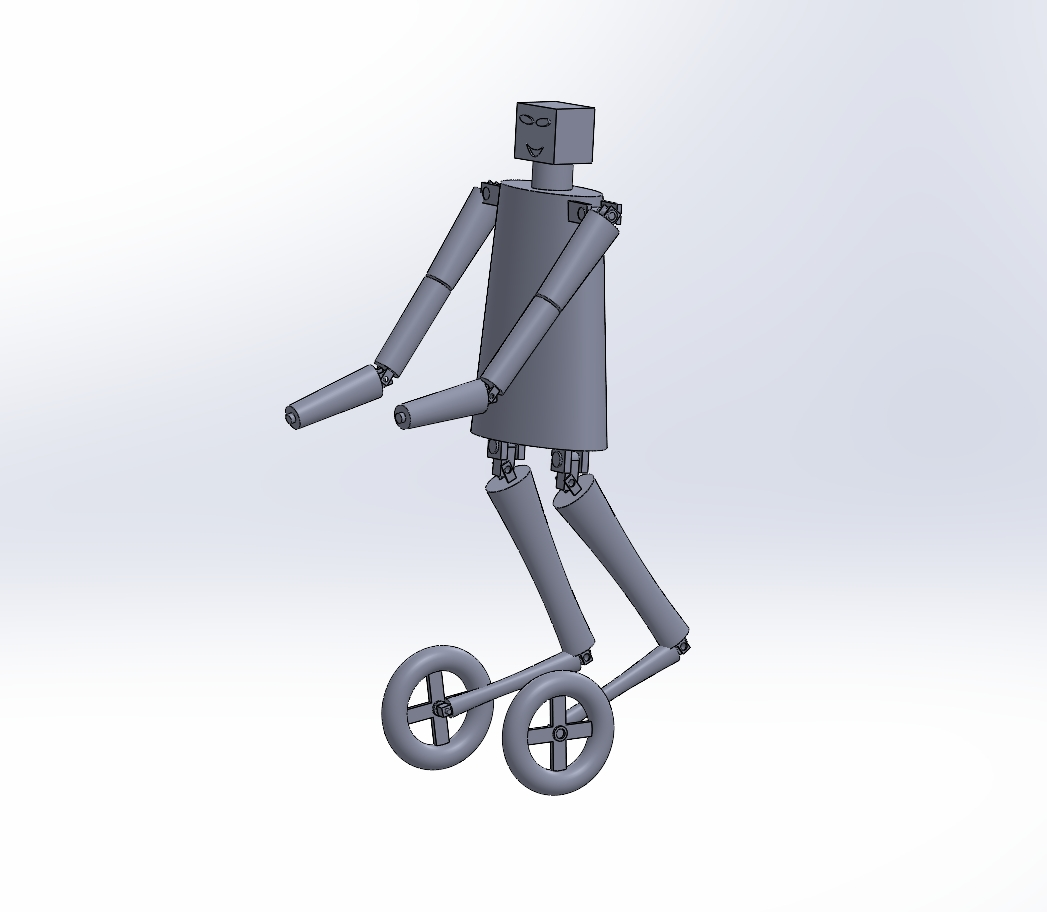
\includegraphics[width=0.3\linewidth]{wheeled_humanoid.png}}
  \subcaptionbox{Roller humanoid\label{fig:b_roller_humanoid}}
    {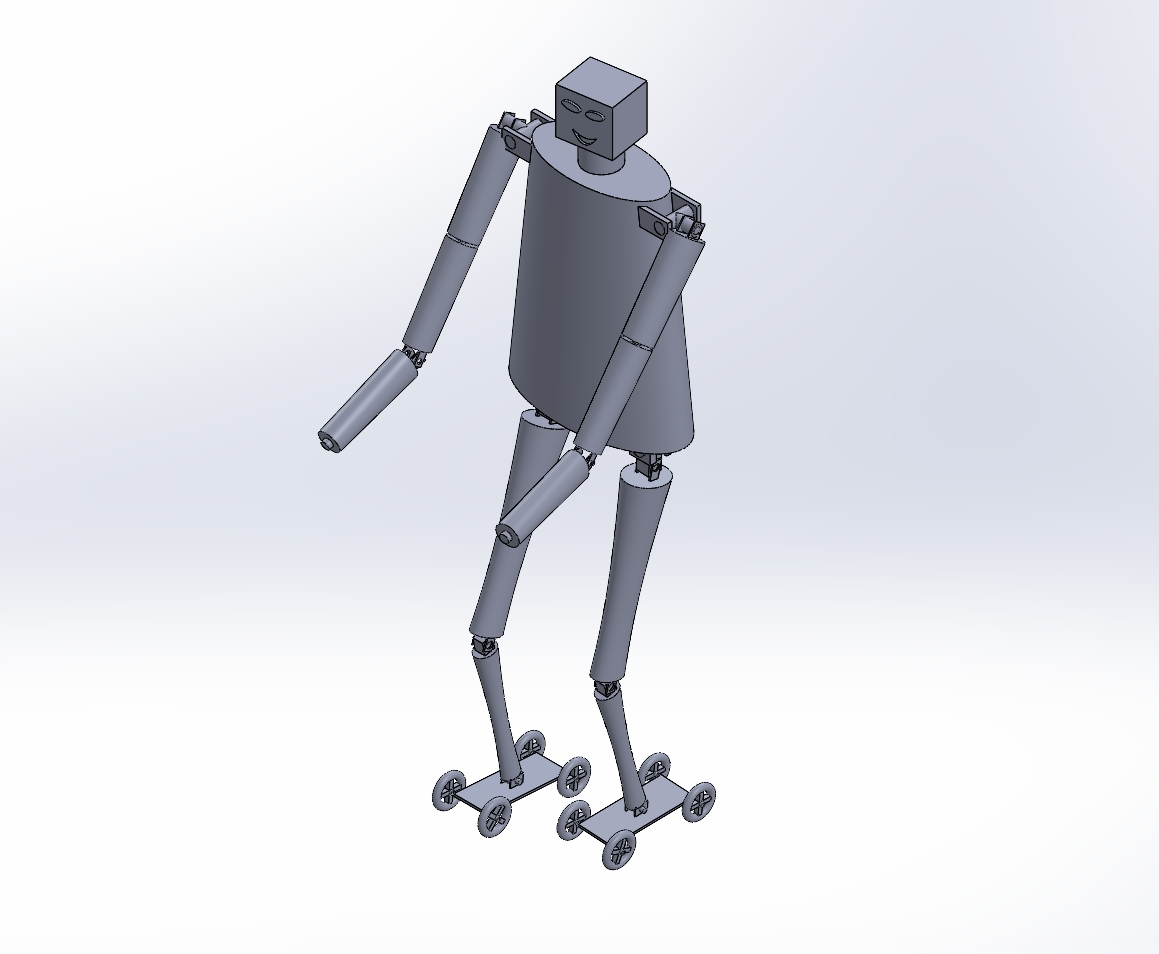
\includegraphics[width=0.3\linewidth]{roller_humanoid.png}}
  \subcaptionbox{wheeled flying\label{fig:c_wheeled_flying}}
    {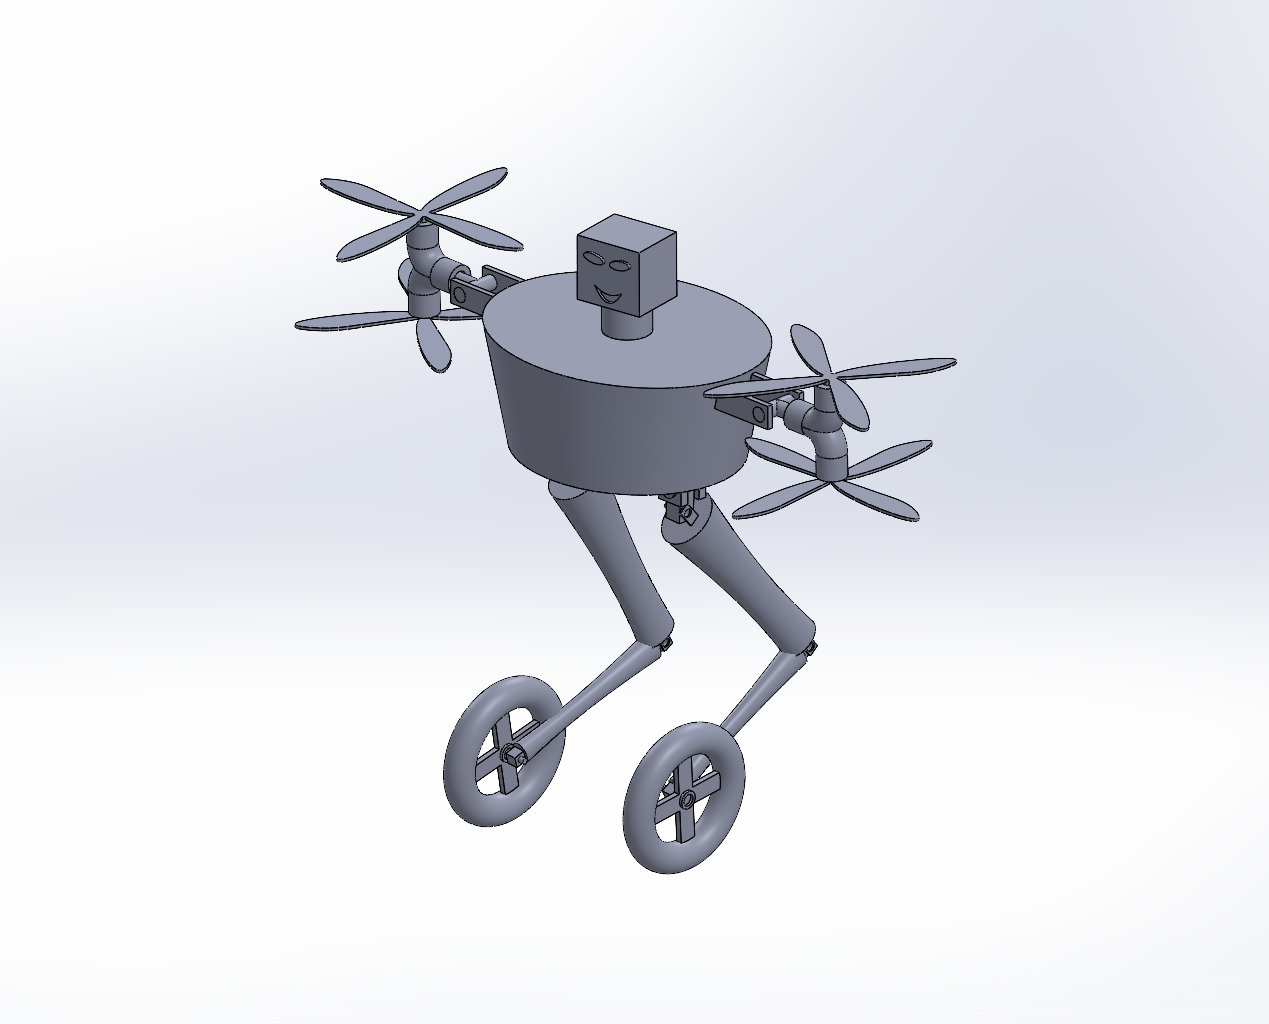
\includegraphics[width=0.3\linewidth]{wheeled_flying.png}}
  % \subcaptionbox{分图 D\label{fig:subfig-d}}
  %   {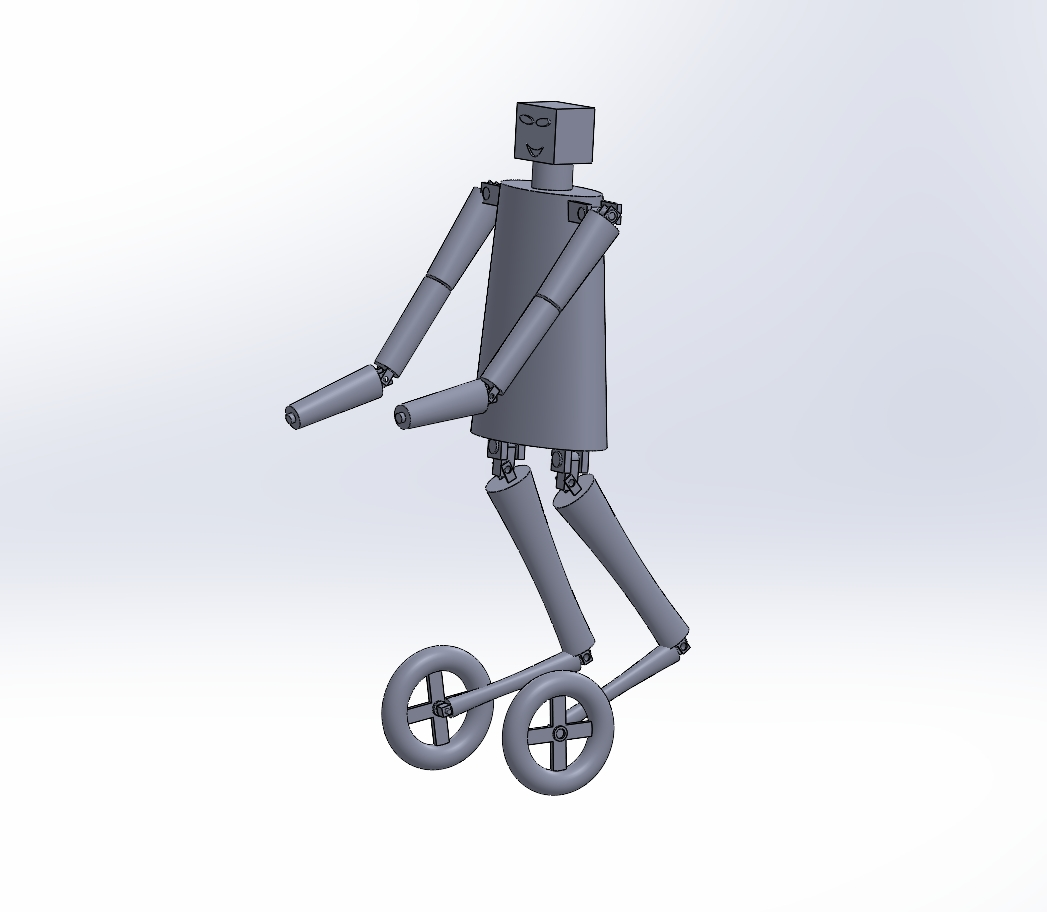
\includegraphics[width=0.45\linewidth]{wheeled_humanoid.png}}
  \caption{三种构想机器人类型的示意图汇总}
  \label{fig:multi_image}
\end{figure}

如图\ref{fig:multi_image}所示,这里给出几种近来构想的机器人结构草图和简单介绍,可以作为随后研究的机器人备选平台参考。

\section[弹跳轮足+机械手机器人]{弹跳轮足+机械手机器人}
如图\ref{fig:wheeled_humanoid}所示,该类型的机器人由类似于Ascento\cite[p1]{Klemm_Morra_Salzmann_Tschopp_Bodie_Gulich_Kung_Mannhart_Pfister_Vierneisel_et_al_2019}类型机器人的双轮足,在此基础上添加两个机械臂构成类人形机器人。该类型的机器人可以轮式地行走和跳跃,同时可以用机械臂模仿双手进行各种操作。

% \textcolor{red}{\small
% 待补充示意图片...
% }
\begin{figure}
  \centering
  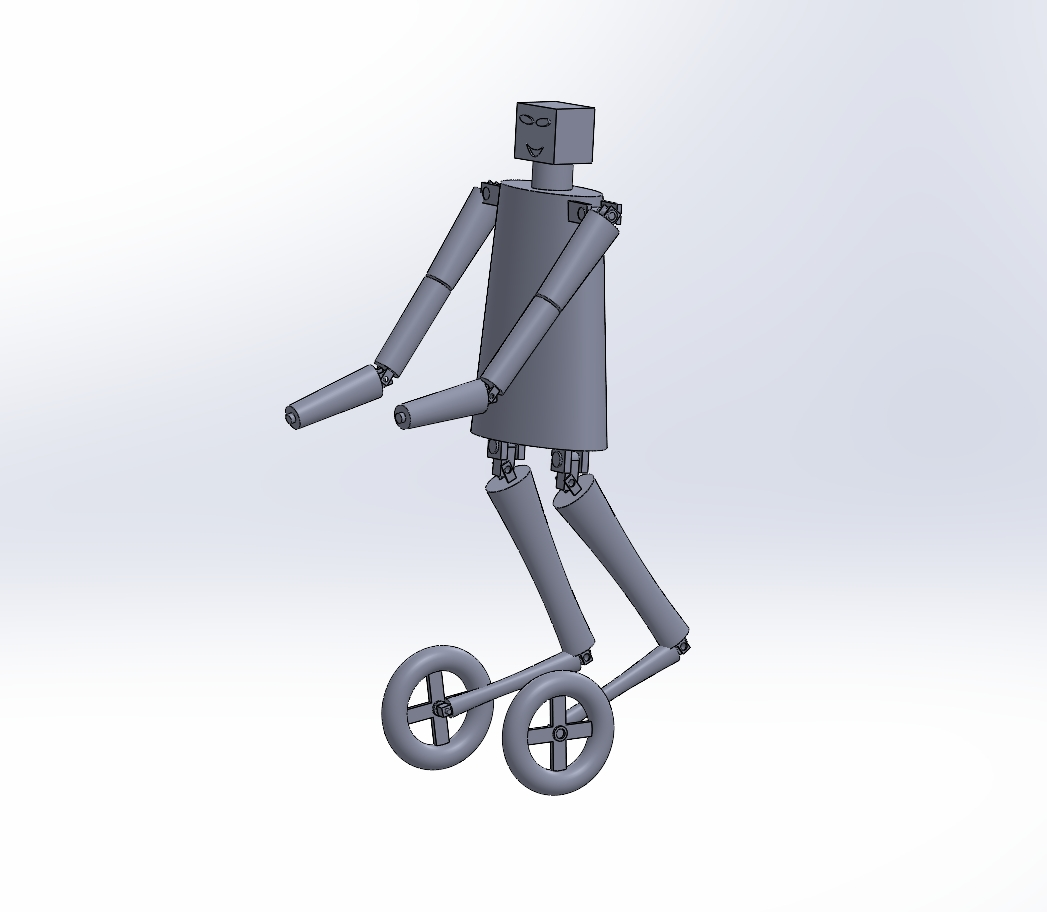
\includegraphics[width=0.6\linewidth]{wheeled_humanoid.png}
  \caption[wheeled_humanoid]{Schematic view of wheeled-humanoid robot}
  \label{fig:wheeled_humanoid}
\end{figure}

该类型机器人的控制基础是倒立摆模型和机械臂运动学,它相对于现有双轮机器人,如Ascento\cite[p1]{Klemm_Morra_Salzmann_Tschopp_Bodie_Gulich_Kung_Mannhart_Pfister_Vierneisel_et_al_2019}等,新的控制问题难点是:
\begin{enumerate}
  \item 在机械手运动的同时保持双轮足的稳定,比如从空手到搬起重物的过程;
  \item 如何让手臂配合轮足实现更加灵巧和优雅的动作;
\end{enumerate}

\section[轮鞋足式+机械手机器人]{轮鞋足式+机械手机器人}
如图\ref{fig:roller_humanoid}所示,该类型的机器人由类似一般人形机器人的基本结构,在此基础之上为每个脚添加四个轮子

% \textcolor{red}{\small
% 待补充示意图片...
% }
\begin{figure}
  \centering
  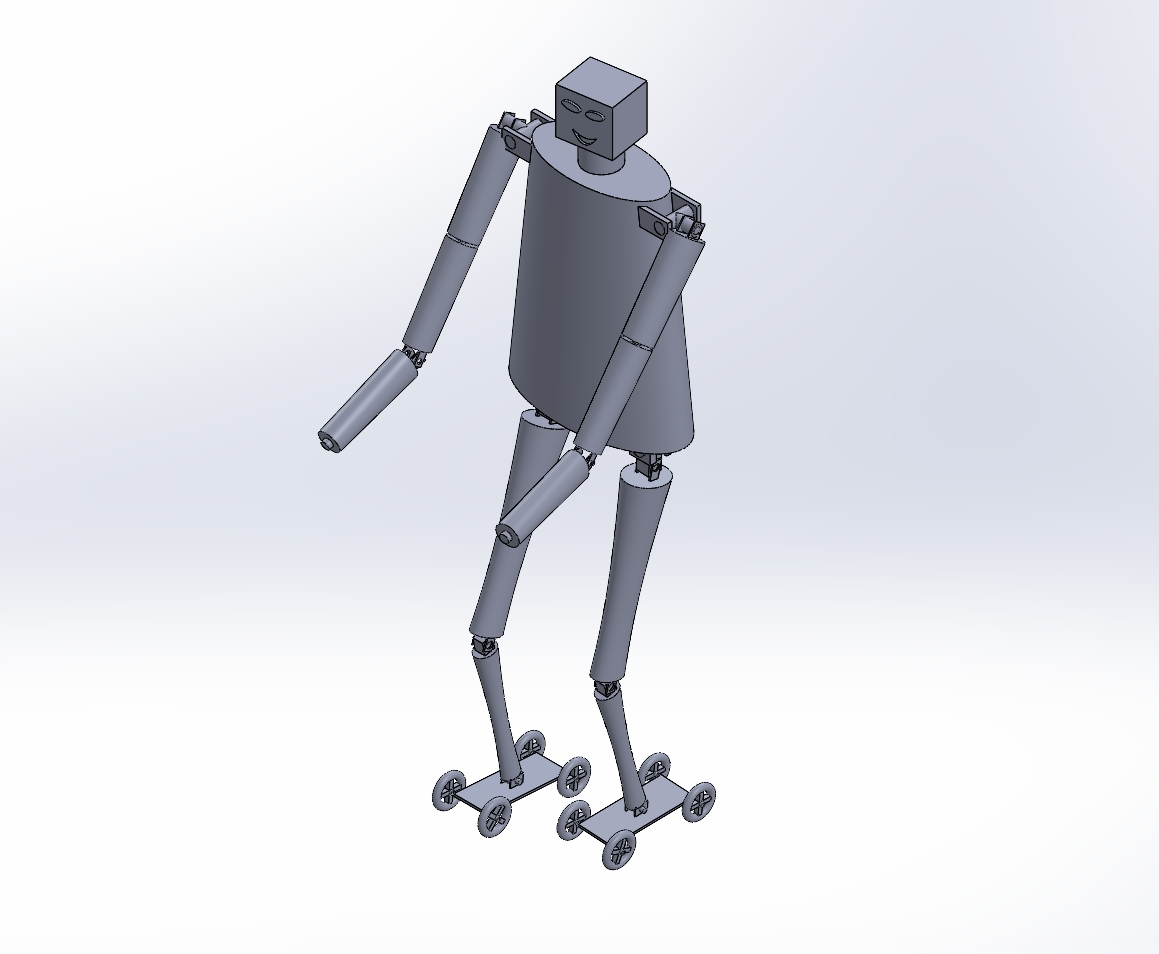
\includegraphics[width=0.6\linewidth]{roller_humanoid.png}
  \caption[roller_humanoid]{Schematic view of roller humanoid.}
  \label{fig:roller_humanoid}
\end{figure}

该类型机器人的控制基础是ZMP约束和机械臂运动学,它相对于现有人形机器人,如\cite[p]{Herzog_Rotella_Schaal_Righetti_2015, Dietrich_Bussmann_Petit_Kotyczka_Ott_Lohmann_Albu_Schäffer_2015}等,新的控制问题难点是:
\begin{enumerate}
  \item 如何实现步态和轮式之间的运动切换;
  \item 如何实现步态和轮式的联合运动平衡;
  \item 在上面两点的基础上,如何结合机械臂实现更加灵巧、优雅、节能的动作;
\end{enumerate}

\section[弹跳轮足+飞行器机器人]{弹跳轮足+飞行器机器人}
如图\ref{fig:wheeled_flying}所示,该类型的机器人由类似于Ascento\cite[p1]{Klemm_Morra_Salzmann_Tschopp_Bodie_Gulich_Kung_Mannhart_Pfister_Vierneisel_et_al_2019}类型机器人的双轮足,在此基础之上添加一对旋翼使其具备飞行能力。

% \textcolor{red}{\small
% 待补充示意图片...
% }
\begin{figure}
  \centering
  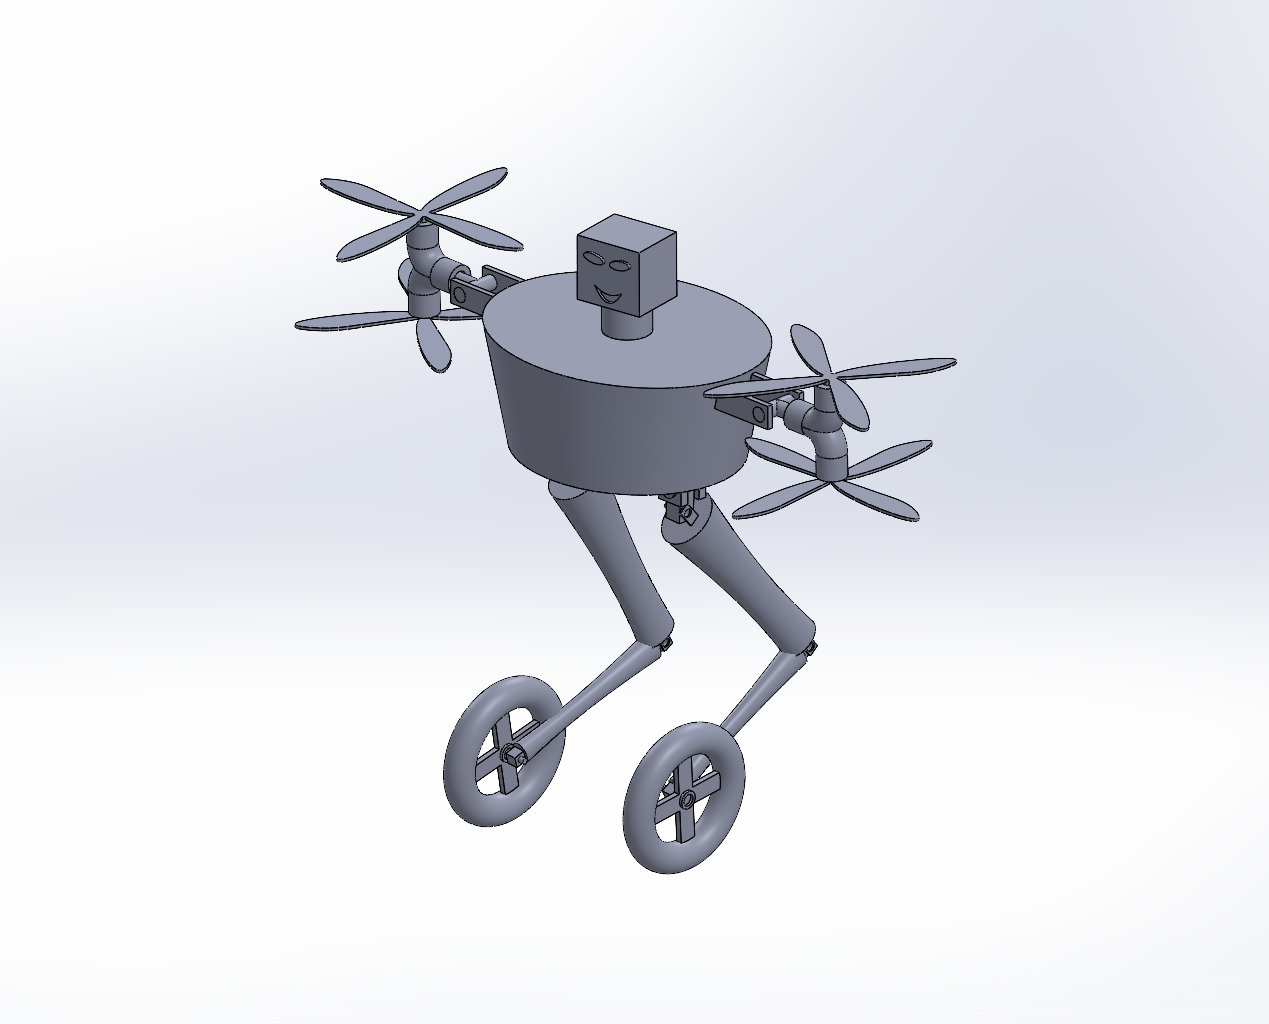
\includegraphics[width=0.6\linewidth]{wheeled_flying.png}
  \caption[short]{Schematic view of wheeled-flying robot.}
  \label{fig:wheeled_flying}
\end{figure}

该类型机器人的控制基础是倒立摆模型和飞行器控制,它相对于现有双轮机器人,如Ascento\cite[p1]{Klemm_Morra_Salzmann_Tschopp_Bodie_Gulich_Kung_Mannhart_Pfister_Vierneisel_et_al_2019}等,新的控制问题难点是:
\begin{enumerate}
  \item 飞行器的矢量控制;
  \item 如何优化设计使得旋翼提供的升力可以满足飞行控制
  \item 续航安全问题;
  \item 如何让旋翼配合轮足实现更加灵巧、优雅、节能、稳定的动作;
\end{enumerate}

% \section[机械狗+飞行器机器人]{机械狗+飞行器机器人}
% 该类型的机器人由类似于ANYmal\cite[p1]{Hwangbo_Lee_Dosovitskiy_Bellicoso_Tsounis_Koltun_Hutter_2019}类型机器人的四足机器人,在此基础之上添加两对旋翼使其具备飞行能力。

% \textcolor{red}{\small
% 待补充示意图片...
% }

% 该类型机器人的控制基础是ZMP约束和飞行器控制,它相对于现有双轮机器人,如Ascento\cite[p1]{Klemm_Morra_Salzmann_Tschopp_Bodie_Gulich_Kung_Mannhart_Pfister_Vierneisel_et_al_2019}等,新的控制问题难点是:
% \begin{enumerate}
%   \item 飞行器的矢量控制;
%   \item 如何优化设计使得旋翼提供的升力可以满足飞行控制
%   \item 续航安全问题;
%   \item 如何让旋翼配合轮足实现更加灵巧、优雅、节能、稳定的动作;
% \end{enumerate}


% % !TeX root = ../sustechthesis-example.tex

\chapter[基于Isaac平台的深度学习训练实践]{基于Isaac平台的深度学习训练实践}

\section[用legged\_gym例程库训练ANYmal-c]{用legged\_gym例程库训练ANYmal-c}

\subsection[训练脚本设置]{训练脚本设置}

\subsection[训练过程信息]{训练过程信息}

\subsection[训练结果输出和重演]{训练结果输出和重演}

\backmatter
% !TeX root = ../sustechthesis-example.tex

\begin{conclusion}

对于经典控制的实现,涉及到复杂的运动模型和动力学建模,难点在于选择优化目标构建优化策略和优化问题的求解。经典控制的优点在于控制过程清晰,可以方便地进行迭代优化和泛化部署;缺点在于建模和实际机器调试复杂,运行时算力开销大。对于强化学习控制的实现,涉及到机器人的仿真模型建模和神经网络设计,难点在于设计合适的优化目标和训练策略以使得训练过程能较快收敛且结果达到预期目标。强化学习控制的优点在于模型设计和调试应用简单迅速,运行时算力开销小;缺点在于控制过程不清晰,导致模型的泛化能力较弱。

经典控制与深度学习控制各有优缺点,在实践应用中两者的有机结合有助于实现更好的控制。在面对一种机器人设计控制策略时,如何分配经典控制和深度学习控制是一个十分重要的问题。两者的融合也是未来的重要发展方向之一。


\end{conclusion}

% 参考文献
\bibliography{ref/refs}  % 参考文献使用 BibTeX 编译
% \printbibliography       % 参考文献使用 BibLaTeX 编译(兼容性不佳,不太推荐)

% 附录
\appendix
% % !TeX root = ../sustechthesis-example.tex

\chapter{补充内容}

附录是与论文内容密切相关、但编入正文又影响整篇论文编排的条理和逻辑性的资料,例如某些重要的数据表格、计算程序、统计表等,是论文主体的补充内容,可根据需要设置。


\section{图表示例}

\subsection{图}

附录中的图片示例(图~\ref{fig:appendix-figure})。

\begin{figure}
  \centering
  
\includegraphics[width=0.6\linewidth]{example-image-a.pdf}
  \caption{附录中的图片示例}
  \label{fig:appendix-figure}
\end{figure}


\subsection{表格}

附录中的表格示例(表~\ref{tab:appendix-table})。

\begin{table}
  \centering
  \caption{附录中的表格示例}
  \begin{tabular}{ll}
    \toprule
    文件名          & 描述                         \\
    \midrule
    sustechthesis.dtx   & 模板的源文件,包括文档和注释 \\
    sustechthesis.cls   & 模板文件                     \\
    thuthesis-*.bst & BibTeX 参考文献表样式文件    \\
    thuthesis-*.bbx & BibLaTeX 参考文献表样式文件  \\
    thuthesis-*.cbx & BibLaTeX 引用样式文件        \\
    \bottomrule
  \end{tabular}
  \label{tab:appendix-table}
\end{table}


\section{数学公式}

附录中的数学公式示例(公式\eqref{eq:appendix-equation})。
\begin{equation}
  \frac{1}{2 \uppi \symup{i}} \int_\gamma f = \sum_{k=1}^m n(\gamma; a_k) \mathscr{R}(f; a_k)
  \label{eq:appendix-equation}
\end{equation}


\section{源代码}

附录中的代码示例:
% 代码\ref{lst:appendix-sample-code-minted},
代码\ref{lst:appendix-sample-code-listings}。

% \begin{listing}[!ht]
% \caption{C++ 代码示例(使用 \pkg{minted} 高亮)}
% \label{lst:appendix-sample-code-minted}
% \begin{minted}[xleftmargin=20pt,linenos]{cpp}
% #include <cstdio>
% #include <cstdlib>
% #include <iostream>
% using namespace std;
% unsigned short i;
% int main() {
%   for (i = 0; i <= 5; i++) {
%     // whatever
%   }
%   return 0;
% }
% \end{minted}
% \end{listing}

\noindent% 取消 minipage 的缩进
\begin{minipage}{\linewidth}
\begin{lstlisting}[language=java,caption={Java 代码示例(使用 \pkg{listings} 高亮)},xleftmargin=20pt,label={lst:appendix-sample-code-listings}]
class HelloWorldApp {
    public static void main(String[] args) {
        System.out.println("Hello World!"); // Display the string.
        for (int i = 0; i < 100; ++i) {
            System.out.println(i);
        }
    }
}
\end{lstlisting}
\end{minipage}

\section{伪代码}

附录中的伪代码示例(算法\ref{algo:appendix-sample-pseudocode})。

\begin{algorithm}
  \caption{Simulation-optimization heuristic}
  \label{algo:appendix-sample-pseudocode}
  \KwData{current period $t$, initial inventory $I_{t-1}$, initial capital $B_{t-1}$, demand samples}
  \KwResult{Optimal order quantity $Q^{\ast}_{t}$}
  $r\leftarrow t$\;
  $\Delta B^{\ast}\leftarrow -\infty$\;
  \While{$\Delta B\leq \Delta B^{\ast}$ and $r\leq T$}{$Q\leftarrow\arg\max_{Q\geq 0}\Delta B^{Q}_{t,r}(I_{t-1},B_{t-1})$\;
  $\Delta B\leftarrow \Delta B^{Q}_{t,r}(I_{t-1},B_{t-1})/(r-t+1)$\;
  \If{$\Delta B\geq \Delta B^{\ast}$}{$Q^{\ast}\leftarrow Q$\;
  $\Delta B^{\ast}\leftarrow \Delta B$\;}
  $r\leftarrow r+1$\;}
\end{algorithm}


\end{document}
